\documentclass[a4paper,11pt]{report}

\author{Florian~Hirtz}
\title{DUMMY: Entwicklung einer Applikation für Mobiltelefone zur Vermittlung von Nachhilfe}

\usepackage[ngerman]{babel}
\usepackage[utf8]{inputenc}
\usepackage[export]{adjustbox}[2011/08/13]
\usepackage{minted}
\usepackage{caption}

\newenvironment{code}{\captionsetup{type=figure}}{}
%\SetupFloatingEnvironment{listing}{name=Source Code}
%Linux
%\usepackage[latin1]{inputenc}
\usepackage{blindtext}
\usepackage{graphicx}
%\usepackage{xcolor}

%minimale page header & footer
\usepackage{fancyhdr}
\pagestyle{fancy}
\setlength{\headheight}{14pt} 
\fancyhf{}
\fancyhead[C]{\nouppercase{\leftmark}}
\fancyfoot[C]{\thepage}

%Depth of sections
\setcounter{secnumdepth}{3}
\setcounter{tocdepth}{3}
\bibliographystyle{abbrv}

%links
\usepackage{hyperref}

\begin{document}
	\maketitle	
	%VORWORT
	\section*{Vorwort}
	Diese Arbeit befasst sich mit der Entwicklung einer Applikation für Mobiltelefone. Die Applikation soll die Vermittlung Nachhilfe unter Schülerinnen und Schüler einer Schule vereinfachen. Dabei ist anzumerken, dass die vollständige Entwicklung einer vollständig markttauglichen Applikation den Rahmen dieser Arbeit sprengen würde. Das Ziel ist vielmehr das legen eines Grundsteins, aus welchem theoretisch ein solches Produkt entstehen könnte.
	\subsubsection*{Zu mir}
	Ich möchte and dieser Stelle die Gelegenheit ergreifen, ein paar Worte zu mir, dem Autor und Entwickler dieser Arbeit, zu verlieren.
	
	Zum Zeitpunkt, an welchem ich begonnen habe, diese Applikation zu entwickeln habe ich zuvor noch nie eine Applikation für Mobiltelefone entwickelt. Bis zu diesem Zeitpunkt hin habe ich mich hauptsächlich auf die Entwicklung kleiner Programme für Computer beschränkt. Das dazu nötige Wissen habe ich mir grösstenteils selber angeeignet. So kommt es auch, das ich vor diesem Projekt mich noch nie gross mit Datenbanken oder Webdevelopement befasst habe. Ich habe mir dieses Projekt als eine Herausforderung genommen, um etwas neues zu lernen und mich als Entwickler zu verbessern. Dieser Lernprozess hat definitiv stattgefunden. Jedoch sollte man sich als Leser/Leserin diese Tatsache immer im Kopf behalten, wenn man sich teile dieser Arbeit ansieht. Oftmals sind Dinge in der Applikation nicht optimal gelöst, teilweise sind gleiche Probleme an verschiedenen Orten verschieden gelöst und weichen oft von anerkannten Praktiken etwas ab.
	\subsubsection*{Motivation}
	Die Motivation, genau eine solche Applikation zu entwickeln kommt hauptsächlich aus zwei Quellen. Zum einen war es der Wille, neue Teilgebiete des Programmierens kennenzulernen und zu verstehen, weshalb die Wahl dann sehr schnell auf eine Applikation für Mobiltelefone viel. Immerhin sind Mobiltelefone in der heutigen Welt kaum mehr wegzudenken und die Fähigkeit, Programme für sie zu entwickeln mich schon länger fasziniert hat. Die zweite Motiviation kam dann von einer Idee von Herrn Bättig, der während der einführenden Präsentation in die Maturarbeit mehr im Witz eine Applikation zur Vermittlung für Nachhilfe erwähnte. Zuerst war ich skeptisch doch schnell stellte ich im Gespräch mit anderen fest, dass eine gut Entwickelte Applikation in diesem Bereich durchaus Verwendung und Beliebtheit finden könnte.
	\subsubsection*{Danksagungen}
	Ich möchte mich hier bei den Personen bedanken, die mich während dieser Arbeit unterstützt haben. Zuerst einmal möchte ich meinem Onkel Peter Arrenbrecht für den Hinweis auf die Firebase API danken, welche mir komplett neue Möglichkeiten geöffnet hat. Weiter möchte ich ein Dankeschön an meine betreuende Lehrperson Andreas Umbach richten, der mir nicht nur einen Platz auf der Datenbank des Ergänzungsfaches zur Verfügung gestellt hat, sondern mir auch immer bei Allfälligen Fragen und Unklarheiten nach seinem Vermögen weitergeholfen hat. Als letztes gilt noch ein gigantisches Dankeschön an meinen Vater, der mich während dieser ganzen Arbeit als Ratgeber und Korrekturleser immer unterstützt hat und immer ein offenes Ohr für meine momentanen Probleme gezeigt hat.

	\tableofcontents
	
	
	%Einleitung
	\chapter{Einleitung}
		\section{Zielsetzung}
		Das Ziel dieser Arbeit ist das Entwickeln einer Applikation für Android Geräte, die die Vermittlung von Nachhilfe unter Schülerinnern und Schülern vereinfachen soll. Die Benutzerinnen und Benutzer der Applikation sollen in der Lage sein, sich einen Account innerhalb der Applikation zu erstellen und sich darin einzuloggen. Sie sollen angeben können, in welchen Fächern sie in der Lage sind, anderen Nachhilfe zu geben. Weiter soll eine Funktion vorhanden sein, mit welcher nach anderen Benutzern gesucht werden kann, die in den gewünschten Fächern Nachhilfe anbieten. So sollen Benutzerinnen und Benutzer bei Bedarf gezielt nach Nachhilfelehrern suchen können, die ihren Bedürfnissen entsprechen. Weiter soll es ihnen möglich sein, über eine Chatfunktion andere Benutzer zu kontaktieren.
	
	%Konzeptionelle Grundlagen
	\chapter{Konzeptionelle Grundlagen} \label{konzepte}
		\section{Client-Server Prinzip}
		Das \emph{Client-Server Prinzip} ist ein weit verbreitetes Konzept, um die Aufgaben innerhalb eines Netzwerkes effizient aufzuteilen. Dabei werden die Aufgaben auf zwei im Netzwerk agierende Programme aufgeteilt. Diese Programme werden im Allgemeinen als Client und Server bezeichnet.
	 
		Der \emph{Server} hat die Aufgabe, verschiedenste Dienste zur Verfügung zu stellen, welche auf Anfrage ausgeführt werden können. Ein solcher Dienst kann zum Beispiel das Versenden einer Nachricht oder das Aufrufen einer Webseite sein. Der Server selbst ist passiv. Ein Server sollte immer in der Lage sein, Anfragen entgegenzunehmen und zu verarbeiten.

		Der \emph{Client} selber ist die aktive Komponente des Systems. Er ist in der Lage, Anfragen an den Server zu stellen und von dessen Diensten Gebrauch zu machen.
		Grundsätzlich gibt es in einem solchen Netzwerk nur einen Server, jedoch kann es durchaus mehrere Clients geben. Ein guter Server sollte also auch darauf vorbereitet sein, mehrere Anfragen von verschiedenen Clients parallel zu bearbeiten. \cite{fachadmin.de:ServerClient}
		
		%TODO BILD VON SCHEMA SERVER-CLIENT
		
		\section{Das Modell-View-Presenter Konzept (Passive View)} \label{mvp}
		Das \emph{Modell-View-Presenter} (MVP) Konzept wie auch auch das sehr ähnliche \emph{Modell-View-Controller} (MVC) Konzept, sind beide für das Entwickeln von Software entworfen worden. Ihre Idee ist es, die Aufgabenbereiche innerhalb einer Applikation strikt voneinander zu trennen. Dabei wird zwischen drei Typen von Aufgabenbereichen unterschieden:
		\begin{itemize}
			\item Die \emph{View} ist die sichtbare Benutzeroberfläche. Sie hat die Aufgabe, dem Benutzer ein bedienbares Interface zu bieten und soll auf Anfrage den Status seiner einzelnen Komponenten weitergeben . Sie kennt das Model nicht.
			\item Das \emph{Model} ist der Datenspeicher einer Applikation, der gebraucht wird um die View korrekt darzustellen. Es soll auf Anfrage hin Daten ausgeben können. In diesem Falle kennt das Model weder die View noch den Presenter. Je nach Auslegung des Konzepts hat das Model jedoch auch die Aufgabe, falls sich Datensätze ändern, den Presenter davon zu unterrichten. Das Model kennt in diesem Falle zwar das Model, jedoch die View nicht.
			\item Der \emph{Presenter} oder \emph{Controller} ist sozusagen der Mittelmann der beiden anderen Komponenten. Er ist in der Lage Daten aus dem Model anzufordern und kontrolliert anschliessend, was mit diesen Daten geschieht. Er hat ebenfalls die Möglichkeit, die angezeigte View zu ändern und deren Status abzufragen. Der Presenter ist in der Lage, sowohl die View zu manipulieren, als auch das Model.
		\end{itemize}
		Wichtig bei dem MVP Konzept mit einem passiven View ist es, dass nur der Presenter die Möglichkeit hat, auf die beiden anderen Komponenten zuzugreifen. Der View und das Model sollen unter keinen Umständen direkt miteinander kommunizieren. Sämtlicher benötigter Informationsaustausch soll stets vom Presenter kontrolliert werden.\cite{mvp} Ein grosser Vorteil einer nach diesen Regeln entwickelter Applikation ist, dass die einzelnen Komponenten weitgehend unabhängig von einander sind. Somit kann zum Beispiel der View komplett neu gestaltet werden, ohne dass der Presenter oder das Modell geändert werden müssen, damit die Applikation weiterhin funktioniert.
		
		\section{Das Hashing und Salzen von Passwörtern}
		
		%TODO BILD VON MVP MODELL
		
	\chapter{Die entwickelte Applikation}
	Die im Rahmen dieser Arbeit entwickelte Applikation wurde für Mobiltelefone mit einer Version des Betriebssystems Android entwickelt. Sie kann darauf installiert und anschliessend ausgeführt werden. Für den Gebrauch der Applikation ist eine Verbindung zum Internet notwendig.
	
	\section{Features}
	Damit die Applikation auch die aufgegebenen Aufgaben erfüllen kann, besitzt sie eine Reihe von Features von welchen Benutzer/Benutzerinnen Gebrauch machen können.
	
	\begin{itemize}
		\item Das \emph{Account-Feature}: Die Applikation bietet den Benutzern/Benutzerinnen die Möglichkeit, sich einen persönlichen Account zu erstellen und ihn zu personalisieren. Es ist ihnen möglich, auf ihrem Profil ihren Namen, ihre besuchte Schule und ihr Geburtsjahr anzugeben. Weiter können sie auch eine kurze Beschreibung von sich selber schreiben und sie haben die Möglichkeit, falls sie selber Nachhilfe anbieten wollen, Fächer auszuwählen, in welchen sie das tun möchten. Das Profil selber ist für andere Benutzer/Benutzerinnen einsehbar. Die meisten Accountdetails können über die Applikation auch noch nach der Registrierung bearbeitet werden.
		\item Das \emph{Such-Feature}: Es ist registrierten Benutzern/Benutzerinnen möglich, über eine Suchfunktion nach anderen registrierten Benutzern/Benutzerinnen zu suchen. Dabei kann nach dem Namen oder nach ausgewählten Fächern gesucht werden. Die gefundenen Profile der verschiedenen Benutzern/Benutzerinnen können anschliessend angesehen werden.
		\item Das \emph{Chat-Feature}: Sollte der Benutzer/die Benutzerin einen anderen Benutzer oder Benutzerin gefunden haben, mit welchem/welcher er/sie Kontakt aufnehmen möchte, so kann ein neuer Chat via das gefundene Profil geöffnet werden. Darin können Benutzer/Benutzerinnen in Echtzeit kurze Textnachrichten miteinander austauschen. Sollte ein Chat geöffnet sein, kann sowohl der Sender/die Senderin wie auch der Empfänger/die Empfängerin ganz einfach von ihrem eigenen Profil auf ihn zugreifen.
	\end{itemize}

	\section{Die entwickelte Applikation}%TODO PROFILBILD WIRD HIER VORAUSGESTEZT + SCREENSHOT VON MAINPAGE, CHAT, SUCHE, PROFIL, LOGIN UND REGISTER
	Wenn die Applikation auf dem Mobilgerät ausgeführt wird, öffnet sich der Login-Screen (siehe Abbildung \ref{}). Der Benutzer/Die Benutzerin kann sich nun hier, sollte er/sie bereits einen Account besitzen, mit seinem/ihrem Benutzernamen und Passwort einloggen. Sollte die Person noch keinen Account besitzen, kann sie über einen Schriftzug unterhalb der Logindaten zu einem Registrierungsformular gelangen (siehe Abbildung \ref{}). Im Registrierungsformular wird nach sämtlichen Daten gefragt, die benötigt werden, um einen Account zu erstellen. Dazu gehört ein Benutzername, Vor- und Nachname, eine E-Mail Adresse, ein Passwort, ein Geburtsdatum sowie die momentan besuchte Schule. Ist die Registrierung erfolgreich, kann der Benutzer/die Benutzerin ab sofort sich in seinen/ihren neuen Account einloggen. Nach dem erfolgreichem Einloggen öffnet sich die Hauptseite der Applikation. Sie besteht hauptsächlich aus dem Profil des Benutzers/der Benutzerin (siehe Abbildung \ref{}). Standardmässig findet sich hier ein Profilbild, der Name des Benutzers/der Benutzerin, sein/ihre Geburtsjahr und die besuchte Schule. Diese und noch weitere Angaben wie angebotene Fächer, eine Beschreibung oder ein Profilbild können in den Einstellungen jederzeit konfiguriert werden, welche über eine Schaltfläche in der oberen rechten Ecke erreicht werden können. Das Profilbild kann dabei entweder direkt mit der Kamera aufgenommen oder aus der Galerie ausgewählt werden. Anschliessend kann der Benutzer/die Benutzerin einen gewünschten ausschnitt im Bild definieren, auf welchen das Bild dann zugeschnitten wird (siehe Abbildung \ref{}). Die ausgewählten Fächer werden in Form von Emblems auf dem Profil dargestellt. Ebenfalls auf der Hauptseite findet sich ein ausfahrbares \emph{BottomSheet} am unteren Ende des Bildschirms. Es kann über eine runde Schaltfläche in der Mitte oder ein einfaches Streichen nach oben ausgefahren werden. Im BottomSheet selber finden sich Einträge für alle offenen Chats des Benutzers/der Benutzerin(siehe Abbildung \ref{}). Über einen einfachen Klick können sie geöffnet werden. Das ist auch der Ort, an welchem ein Benutzer/eine Benutzerin sehen kann, ob er/sie neue Nachrichten empfangen hat. Neben dem BottomSheet findet sich ebenfalls im rechten unteren Ende eine runde Schaltfläche mit einer Lupe. Über sie kann auf das Such-Feature zugegriffen werden, welche den Benutzer/die Benutzerin auf einen neuen Screen führt. Dort können die Kriterien für die Suche definiert werden (siehe Abbildung \ref{}). Hier können Suchparameter wie Name und Fächer angegeben werden, nach welchen gesucht werden soll. Ist der Benutzer/die Benutzerin zufrieden mit den Einstellungen kann über eine Schaltfläche die Suche ausgeführt werden. Alle Suchergebnisse werden in Form einer Liste daraufhin im Client aufgeführt. Sollte den Benutzer/die Benutzerin Interesse an einem der Ergebnisse haben, kann durch einfaches Auswählen des Elementes in der Liste das Profil des/der gefundenen Benutzer/Benutzerin aufgerufen werden (siehe Abbildung \ref{}). Ist der Benutzer/die Benutzerin interessiert, Kontakt mit dem/der gefundenen Benutzer/Benutzerin aufzunehmen, kann nun über eine Schaltfläche auf dem Profil ein neuer Chat geöffnet werden (siehe Abbildung \ref{}). Dort können dann mithilfe kurzer Textnachrichten genauere Informationen über eine mögliche Zusammenarbeit ausgetauscht werden. Die Überlieferung erfolgt dabei in Echtzeit.
	
	%Projektentwicklung
	\chapter{Applikationskomponenten}
	In diesem Kapitel wird verwendete Komponenten innerhalb der Applikation eingegangen. Die einzelnen Komponenten sollen erklärt werden und ihre Rolle in der entwickelten Applikation ersichtlich werden.
		\section{Systemüberblick}
		Die Applikation basiert auf dem Client-Server Prinzip. Der Client findet sich in Form der entwickelten Anwendung, die auf Mobiltelefonen von den Benutzern/Benutzerinnen installiert werden kann. Der Server wird von den beiden Datenbanken gebildet. Die Interaktionen der einzelnen Komponenten entsprechen weitgehend dem MVP Konzept (siehe Kapitel \ref{konzepte}). Der Presenter und die View finden sich beide auf Seiten des Clients (siehe Kapitel \ref{client}) während das Model sich in Form der beiden Server wiederfindet (siehe Kapitel \ref{server} und \ref{fb}).
		
		%Die Server
			\section{Datenbank Server} \label{server}
			Eine der wohl wichtigsten Aufgaben von Computern ist das Speichern, Verwalten und auch Manipulieren von Informationen. Anwendungen, die sich hauptsächlich mit dieser Aufgabe beschäftigen werden allgemein als \emph{Datenbanken} bezeichnet. Sie haben die Aufgabe, Informationen systematisch zu ordnen, zu speichern und bei Bedarf zu verändern. Grundsätzlich bezeichnet der Begriff Datenbank gleich zwei Dinge auf einmal. Zum einen wird ein strukturierter Speicher von Informationen als Datenbank bezeichnet und zum anderen jedoch auch die Anwendung, die das Verwalten der Daten überhaupt erst ermöglicht. Solche Anwendungen werden genauer als \emph{Database Management System} (DBMS) bezeichnet und sind meist hochkomplex in ihren Funktionsweisen, um selbst die effiziente Verwaltung von riesigen Datenmengen zu ermöglichen. \cite{IT-Handbuch}
			
			Die Informationen werden in einer Datenbank meist in Form von Tabellen gespeichert. Dabei wird eine einzelnen Zeile in der Tabelle als Datensatz oder Eintrag bezeichnet, während die verschiedenen Spalten Felder genannt werden. Beim erstellen einer solcher Tabelle werden zuerst die verschiedenen Felder bestimmt. Ihnen wird ein Name gegeben, der beschreibt, was darin gespeichert werden soll. Hinzu kommt ein Datentyp, der angibt um was es sich bei diesem Feld handelt (z.B. eine Zahl oder einen kurzen Text). Es ist ebenfalls möglich einem Feld einen Default Wert zuzuschreiben. Dieser wird dann für einen Datensatz verwendet, wenn das Feld sonst nicht definiert wurde. Zuletzt ist es noch möglich, einem Feld speziellere Eigenschaften zuzuschreiben. Dazu gehört unter anderem eine Funktion mit dem Name \emph{auto\_increment}. Sie bewirkt bei einem Feld des Datentypen Integer, das beim Erfassen eines neuen Datensatzes automatisch in diesem Feld die Position des Datensatzes in der Tabelle dafür verwendet werden soll. 
			
			Datenbanken selber können in verschiedene Typen eingeteilt werden, die alle ihre eigenen Vor- und Nachteile mit sich bringen. Die einfachste Form eines Datenbanktyps ist wohl die \emph{Einzeltabellendatenbank}. Sie besteht aus nur einer Tabelle, in welcher alle Informationen abgespeichert werden. Sie eignet sich gut für kleine, übersichtliche Tabellenstrukturen wie zum Beispiel eine einfache Liste von Adressen. Die Einzeltabellendatenbank stösst jedoch spätestens dann an ihrer Grenzen, wenn die Informationen nicht mehr in nur einer, sondern gleich mehreren Tabellen gespeichert werden sollen. Hier tritt ein anderer Datenbanktyp ins Spiel. Eine \emph{relationale Datenbank} ist in der Lage, verschiedene Tabellen logisch miteinander zu verknüpfen und sich darin zu orientieren. Diese logische Verknüpfung ist möglich aufgrund eindeutiger Eigenschaften eines Datensatzes. Dies kann zum Beispiel eine Kundennummer oder ein Name sein. Ein solches Feld wird auch als ein \emph{Key} bezeichnet. Wichtig dabei ist, dass jeder Key nur einmal in einer Tabelle vorkommt, da ansonsten keine eindeutige Verknüpfungen möglich sind. Die Anwendung zur Verwaltung einer solchen relationalen Datenbank wird \emph{Relational Database Management System} (RDBMS) genannt. \cite[S. 745 - 751]{IT-Handbuch}

				\subsection{MySQL Datenbank}
				%TODO GLOSSARY WORK ON LICENCE
				%TODO MySQL ODER MariaDB
				Ein Beispiel für ein solches RDBMS ist die weit verbreitete MySQL Datenbank. Das System wurde ursprünglich von den drei Gründern Allan Larsson, Michael Widenius und David Axmark 1995 entwickelt, wurde später von \emph{Sun Microsytems} aufgekauft und gelangte schlussendlich in den Besitz des amerikanischen Softwareherstellers \emph{Oracle}. MySQL ist unter einem dualen Lizenzsystem eingetragen, sodass die Software zum einen unter einer \emph{General Public Licence} (GPL), aber auch unter eine proprietäre Lizenz gestellt ist. \cite{tecmint.com} Das MySQL System darf aufgrund der GPL gratis heruntergeladen, installiert und modifiziert werden.
				
				In Kombination mit der Programmiersprache PHP bildet sie eines der meist verwendeten Datenspeichersysteme für Webdienste aller Art. Im Falle eines solchen Webdienstes befindet sich die Datenbank meist auf einem zentralen Server, auf welchem sich ebenfalls die benötigten PHP-Skripte befinden. Die PHP-Skripte haben die Aufgabe, Abfragen von den Clients entgegenzunehmen und über sogenannte \emph{Queries} (Datenbank Abfragen) auf die Informationen in der Datenbank zuzugreifen. Im Falle einer MySQL Datenbank werden solche Queries in der Datenbanksprache \emph{SQL} (Structured Query Language) formuliert. Queries können in vier Arten von Abfragen unterteilt werden: \cite[S. 760]{IT-Handbuch}
				
				\begin{itemize}
					\item Auswahlabfragen (\emph{Select Queries}) geben den Inhalt von einem oder mehreren Feldern aus einer oder verschiedenen Tabellen zurück. Dabei kann bei Bedarf nach Kriterien gefiltert werden, um die Suche nach bestimmten Datensätzen einzugrenzen.\cite[S. 746]{IT-Handbuch}
					\item Einfügeabfragen (\emph{Insert Queries}) fügen einen neuen Datensatz zu einer bestehenden Tabelle hinzu.\cite[S. 746]{IT-Handbuch}
					\item Änderungsabfragen (\emph{Update Queries}) ändern bestimmte oder alle Felder eines bestehenden Datensatzes in einer Tabelle.\cite[S. 746]{IT-Handbuch}
					\item Löschabfragen (\emph{Delete Queries}) löschen einen Datensatz aus einer Tabelle. \cite[S. 746]{IT-Handbuch}
				\end{itemize}
				
				\subsection{MySQL Datenbankstruktur} \label{databankstructure}
				
				\begin{figure}
					\begin{center}
						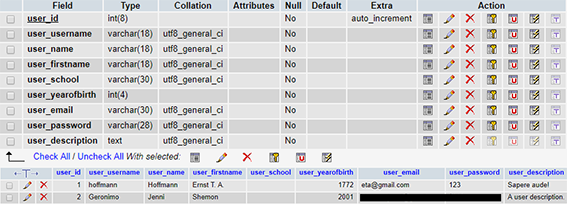
\includegraphics[center]{user_archive.png}
						\caption{Oben: Struktur der user\_archive Tabelle, aufgenommen aus dem phpMyAdmin Interface Unten: Beispielhafter ausschnitt aus der Tabelle selber, aufgenommen aus dem phpMyAdmin Interface}
						\label{user_archive:PNG}
					\end{center}
				\end{figure}
				\begin{figure}
					\begin{center}
						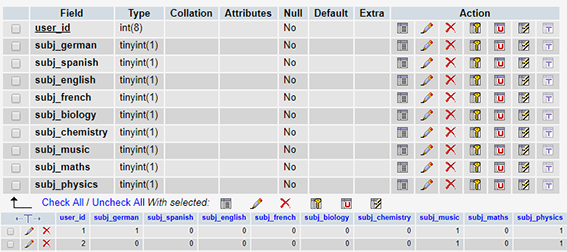
\includegraphics[center]{user_subjects.png}
						\caption{Die user\_subjects Tabelle, aufgenommen aus dem phpMyAdmin Interface}
						\label{user_subjects:PNG}
					\end{center}
				\end{figure}
				\begin{figure}
					\begin{center}
						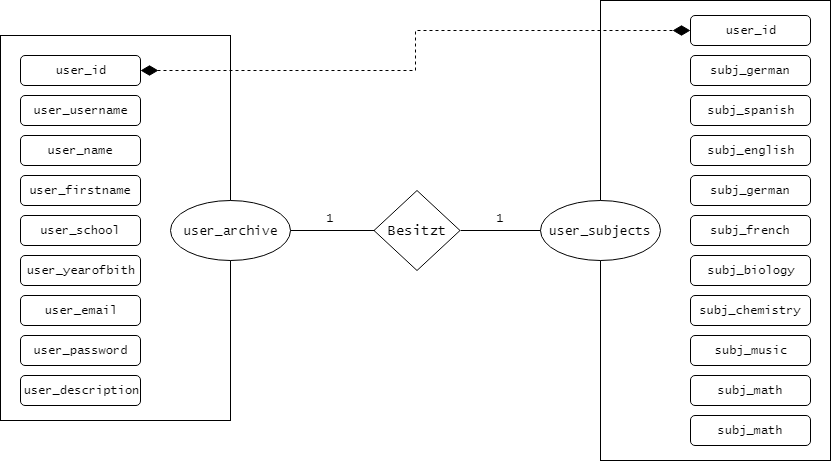
\includegraphics[width=0.8\textwidth]{ERM-Matura.png}
						\caption{Das ERM der entwickelten Applikation.}
						\label{ERM}
					\end{center}
				\end{figure}
				
				%TODO REWRITE AND STRUCTURE
				%In der entwickelten Applikation wird genau ein solches MySQL Datanbanksystem in Kombination mit PHP (siehe Kapitel \ref{ssec:PHP}) benutzt. Die Datenbank wird verwendet, um die Accountdaten der einzelnen Benutzer zu speichern und den Clients zur Verfügung zu stellen. Sie befindet sich auf dem Schulserver vom Ergänzungsfach. Die Datenbank selber umfasst zwei miteinander verknüpfte Tabellen. Die eine läuft unter dem Name \emph{user\_archive} (siehe Abbildung \ref{user_archive:PNG}) und beinhaltet die essentiellen Accountdetails wie Name, Email, Passwort etc. Zu erwähnen ist hier das erste Feld \emph{user\_id}. Es wird bei einem neuen Eintrag in die Tabelle automatisch generiert (\emph{auto\_increment}) und gewährt so, dass sämtliche Einträge eindeutig unterschieden werden können. Ähnlich verhält sich das Feld user\_username. Es ist als \emph{unique} markiert und soll ebenfalls verhindern, dass es beim Login zu Mehrdeutigkeiten kommt. Sie sind die Keys der Tabelle. Die zweite Tabelle der trägt den Namen \emph{user\_subjects} (siehe Abbildung \ref{user_subjects:PNG}). Sie umfasst nebst einem Feld für die user\_id sämtliche momentan von der Applikation unterstützten Fächer. In den Feldern wird nun mithilfe von 1 und 0 angegeben, welche Fächer von einem Benutzer/ einer Benutzerin angewählt wurden, also in welchen er/sie andere unterstützen könnte. Die Inhalte wurden bewusst von einander getrennt, um die Übersichtlichkeit in der user\_archive Tabelle zu wahren. Das user\_id Feld ist auch hier ein Key und ist für jeden Benutzer gleich wie in der user\_archive Tabelle. Diese Verknüpfung der Tabellen kann sehr übersichtlich durch ein \emph{Entity-Relationship-Modell} (ERM) dargestellt werden, da das Modell lediglich zwei Tabellen (Im falle des ERM \emph{Entities}) umfasst. ERMs eignen sich besonders für die Darstellung von Datenbankstrukturen und deren Verknüpfungen. Sie sind oft der erste Schritt, wenn es um die Planung einer neuen Datenbank geht. Die Beziehungen werden durch hauptsächlich zwei Variablen beschrieben, welche im Schema (x, y) dargestellt werden. Die Variable x gibt das Minimum an herrschenden Beziehungen mit anderen Entities vor. Die Variable y das Maximum. Die Variablen können entweder eine bestimmte Zahl wie 1 oder 0 sein oder sie können durch m/n verkörpert werden, stellvertretend für beliebig viele Beziehungen. Im falle des ERMs der entwickelten Applikation (siehe Abbildung \ref{ERM}) ist das eine (1,1) : (1,1) Beziehung. Das bedeutet, dass es in beiden Tabellen jeweils genau einen Eintrag für einen Benutzer gibt. \cite[S. 750]{IT-Handbuch}\cite{ERM}\cite{ERM2}

				In der entwickelten Applikation wird genau ein solches MySQL Datanbanksystem in Kombination mit PHP (siehe Kapitel \ref{ssec:PHP}) benutzt. Die Datenbank wird verwendet, um die Accountdaten der einzelnen Benutzer zu speichern und den Clients zur Verfügung zu stellen. Sie befindet sich auf dem Schulserver vom Ergänzungsfach. Die Datenbank umfasst 4 Tabellen.
				
				\begin{itemize}
					\item Die \emph{user\_archive} Tabelle beinhaltet allgemeine Informationen zu einem Registrierten Benutzer. Dazu gehören Informationen wie Benutzername, Vor- und Nachname, Email, Jahrgang und die momentan besuchte Schule. Zudem kommt noch eine Benutzer ID (\emph{user\_id}), welche jedem Benutzer automatisch über die auto\_increment Funktion beim registrieren zugewiesen wird und daher für jeden Benutzer einzigartig ist. Eine Darstellung der user\_archive Tabelle findet sich in Abbildung \ref{user_archive:PNG}.
					\item Die \emph{user\_profilepicutres} Tabelle besitzt drei Felder. Eines für die user\_id, und zwei Felder vom Datentyp \emph{Medium BLOB}, in welchen jeweils eine kleine und eine grosse Variante des Profilbildes eines Benutzers/einer Benutzerin gespeichert wird. Das speichern von grösseren Bilddateien in Relationalen Datenbanken ist umstritten und man findet hier verschiedene Ansichten. Im Rahmen dieser Arbeit jedoch sollte diese Datenbankkonfiguration keine grösseren Probleme mit sich bringen, weshalb es dann dabei belassen wurde. Mehr dazu in Kapitel \real{}.
					\item Die \emph{user\_hashes} Tabelle besitzt drei Felder. Eines für die user\_id, eines für das gehashte Password und eines für das Salz eines Benutzers/einer Benutzerin. Mehr dazu in Kapitel \ref{}.
					\item Die \emph{user\_subjects} Tabelle beinhaltet Felder für alle von der entwickelten Applikation unterstützten Fächer (siehe Abbildung \ref{user_subjects:PNG}). Mithilfe der Werte 1 und 0 wird angegeben, in welchen Fächern ein Benutzer/eine Benutzerin Unterstützung anbietet.
				\end{itemize}
			
				
				Diese Tabellen können alle über die user\_id eines Benutzers miteinander verknüpft werden. Die user\_id ist zudem in allen Tabellen als ihr jeweiliger \emph{Primary Key} markiert. Für die Datenbank bedeutet dies, das dieses Feld jeweils für jeden Datensatz einen einzigartigen Wert besitzt und für die Unterscheidung der Datensätze optimiert werden soll. Besonders für grosse Datenbanken ist eine geschickte Handhabung solcher Keys von grosser Bedeutung, da sie die Effizienz einer Datenbank drastisch beeinflussen kann.
				
				Die genauere Struktur der gesamten Datenbank kann durch ein \emph{Entitiy-Relationship-Modell} (ERM) dargestellt werden. ERMs sind in der Lage zu visualisieren, in welcher Beziehung verschiedene Bestandteile von Datenstrukturen (\emph{Enities}) zu einander stehen. ERMs sind oftmals der erste Schritt wenn es um die Planung einer neuen Datenbank geht. Das ERM der im Rahmen dieser Arbeit benutzen Datenbank ist in Abbildung \ref{ERM} dargestellt. Die Verhältnisse werden im Schema (1, 1) geschrieben. Die erste Ziffer gibt die minimale Anzahl an herrschenden Beziehungen an, die zweite Ziffer die maximale Anzahl. Im Falle von (1, 1) Beziehungen bedeutet dies, dass es immer genau eine solche Beziehung geben darf und auch muss. Sind die Anzahl Beziehungen unlimitiert, stehen anstelle der Ziffern stellvertretend die Variablen \emph{m} oder \emph{n}. Die Tabellen sind alle über den Key user\_id miteinander Verknüpfbar.\cite[S. 750]{IT-Handbuch} \cite{ERM} \cite{ERM2}
				
				
				%eine \emph{user\_archive} Tabelle, eine user\_profilepictures Tabelle, eine user\_hashes Tabelle und eine \emph{user\_subjects} Tabelle. In der user\_archive Tabelle findet sich ein Eintrag für jeden registrierten Benutzer mit Informationen wie Benutzername, Vor- und Nachname, Email, Jahrgang sowie die momentan besuchte Schule (siehe Abbildung \ref{user_archive:PNG}). Die user\_subjects Tabelle beinhaltet Felder für alle von der entwickelten Applikation unterstützten Fächer (siehe Abbildung \ref{user_subjects:PNG}). Mithilfe der Werte 1 und 0 wird angegeben, in welchen Fächern ein Benutzer/eine Benutzerin Unterstützung anbietet. Die Struktur der Datenbank kann durch ein \emph{Entitiy-Relationship-Modell} (ERM) dargestellt werden. ERMs sollen visualisieren, in welcher Beziehung verschiedene Bestandteile von Datenstrukturen (\emph{Enities}) zu einander stehen. ERMs sind oftmals der erste Schritt wenn es um die Planung einer neuen Datenbank geht. Das ERM der im Rahmen dieser Arbeit benutzen Datenbank ist in Abbildung \ref{ERM} visualisiert. Die Verhältnisse werden im Schema (1, 1) geschrieben. Die erste Ziffer gibt die minimale Anzahl an herrschenden Beziehungen an, die zweite Ziffer die maximale Anzahl. Im Falle von (1, 1) Beziehungen bedeutet dies, dass es immer genau eine solche Beziehung geben darf und auch muss. Sind die Anzahl Beziehungen unlimitiert, steten anstelle der Ziffern stellvertretend die Variablen \emph{m} oder \emph{n}. Die Tabellen sind über den Key user\_id miteinander Verknüpfbar.\cite[S. 750]{IT-Handbuch} \cite{ERM} \cite{ERM2}
				
				%Abbildungen von den beiden Tabellen findet sich in den Abbildungen \ref{user_archive:PNG} und \ref{user_subjects:PNG}. Im oberen Teil der Abbildungen sieht man die Konfiguration der einzelnen Felder. In der Spalte \emph{Field} ist der Name der Felder eingetragen. In der Spalte \emph{Type} wird der zugelassene Datentyp des Feldes definiert. Ist der Datentyp eine Form von Text, wird in der Spalte \emph{Collation} die Kodierung der Unicode-Zeichen angegeben. In der Spalte \emph{Extras} können noch eine Reihe von speziellen Eigenschaften den Feldern zugewiesen werden. Eine davon ist die im Feld \emph{user\_id} verwendete \emph{auto\_increment} Funktion. Sie führt dazu, dass neue Einträge in der Tabelle in diesem Feld automatisch durchnummeriert werden. Das Feld user\_id ist in beiden Tabellen als Key markiert. Das heisst, dass das die user\_id von der Datenbank zur eindeutigen Verknüpfung der beiden Tabellen benutzt werden soll. Ebenfalls zu erwähnen ist das Feld \emph{user\_username}. Es ist als \emph{unique} markiert, was heisst, dass es in der Tabelle keine identische Benutzernamen geben darf (siehe Kapitel \ref{login:php}). 
				
				%Im unteren Teil der Abbildungen findet sich ein beispielhafter Ausschnitt, wie eine solche Tabelle mit ausgefüllten Feldern Aussehen könnte.
				%TODO GLOSSAR OBJEKTORIENTIERT
				\subsection{PHP Skripte} \label{ssec:PHP}
				Nebst dem Datenbanksystem selbst befinden sich ebenfalls diverse PHP Skripte auf dem Server. Sie sind in der Open-Source Skriptsprache PHP geschrieben. PHP ist ein rekursives Akronym für \emph{Hypertext Preprocessor} und ist eine speziell für die Webprogrammierung entwickelte Programmiersprache, welche zu den objektorientierten Programmiersprachen gehört. PHP wird hauptsächlich für die Programmierung innerhalb von Webservern verwendet und bietet den grossen Vorteil, dass Clientbenutzer zwar durchaus die Skripte auf dem Server ausführen, jedoch nicht ansehen können. Sie erhalten lediglich eine Antwort ohne je die Codestruktur des PHP Skriptes zu Gesicht bekommen zu haben.\cite{PHP} Dies ist möglich, da der PHP-Code ausschliesslich serverseitig ausgeführt wird. Ein \emph{Interpreter} führt ihn auf dem Server aus und erst die vom Interpreter generierte Ausgabe wird dem Client als Antwort zugeschickt. Die Antwort ist meist in der Auszeichnungssprache HTML (\emph{Hypertext Markup Language}) verfasst, können jedoch durchaus auch in PDF, JavaScript, JSON oder sogar Bildformaten sein.\cite{PHP:function} Die Website \emph{json.org} (\cite{JSON}) beschreibt JSON wie folgt:
				
				%TODO GLOSSAR PARSEN
				\begin{quotation}
					"JSON (JavaScript Object Notation) ist ein schlankes Datenaustauschformat, das für Menschen einfach zu lesen und zu schreiben und für Maschinen einfach zu parsen (Analysieren von Datenstrukturen) und zu generieren ist.[...]Bei JSON handelt es sich um ein Textformat, das komplett unabhängig von Programmiersprachen ist[...]. Diese Eigenschaften machen JSON zum idealen Format für Datenaustausch."\cite{JSON}
				\end{quotation}
			
				Die im Rahmen dieser Arbeit entwickelte Applikation benutzt für ihre Kommunikation von MySQL Datenbank zu Client ausschliesslich JSON-Formate. Dieses Format eignet sich perfekt für den Austausch von Daten wie sie in der Datenbank gespeichert sind.
				
				%TODO: MB POST ERWÄHNEN BEI ENTGEGENGENOMMENEN BENTZERNAME UND PASSWORT
					\subsubsection{Login}\label{login:php}
					Damit ein Client Zugriff auf einen Datensatz eines Benutzers/einer Benutzerin in der Datenbank bekommt, muss sich der Benutzer/die Benutzerin zuerst unter einem bestehenden Account einloggen. Hierzu muss im Client sowohl der Benutzername wie auch das Passwort eines Registrierten Accounts eingegeben werden. Danach erfolgt das Login in zwei Schritten.
					
					Im ersten Schritt wird vom Client das \emph{salt\_php.php} File auf dem Server vie Webadresse aufgerufen, wobei dem PHP File mithilfe der POST Methode der eingegebene Benutzername übergeben wird. Dort wird dann anschliessend ein sogenanntes \emph{MySQL Statement} erstellt. Solche Statements sind in der Lage, Anfragen an die verbundene Datenbank zu stellen. In diesem Falle wäre das nun eine Auswahlabfrage (Select Query), die in der user\_archive Tabelle nach einem Datensatz mit dem eingegebenen Benutzername sucht, wobei die Tabelle über einen \emph{INNER JOIN} mit der user\_hashes Tabelle verknüpft wird (siehe Abbildung \ref{SQL:SALT}). Dabei darf jeweils nur ein Eintrag gefunden werden, weshalb jeder Benutzername in der Datenbank einzigartig sein muss. Wird ein Datensatz mit dem eingegebenen Benutzernamen gefunden, wird dem Client das Salz des Benutzers/der Benutzerin in JSON-Format zurückgegeben. 
					
					\begin{code}
						\begin{center}
							\begin{minted}[breaklines]{sql}
SELECT user_hashes.hash_salt FROM user_archive INNER JOIN user_hashes ON user_archive.user_id = user_hashes.user_id WHERE user_archive.user_username = ?
							\end{minted}
						\end{center}
					\caption{Select Query für das Auslesen des Salzes eines Benutzers aus der user\_archive Tabelle und der user\_hashes Tabelle.}\label{SQL:SALT}
					\end{code}
					
					%TODO REF HASHING
					Im zweiten Schritt wird auf Seiten des Clients das eingegebene Passwort zusammen mit dem Salz gehasht (siehe Kapitel \ref{}) und der erhaltene Hash wieder an das login\_php\_v2.php File auf dem Server übergeben. Dieses vergleicht nun den erhaltenen Hash mit dem in der Datenbank gespeicherten Hash. Sind beide identisch, wurde das korrekte Passwort eingegeben. Nun können alle benötigten Informationen über den Benutzer aus der Datenbank über eine Auswahlabfrage ausgelesen werden und im JSON-Format an den Client geantwortet und Teilt dem Client darin gleichzeitig noch mit, das dass Login erfolgreich war.
					
					Sollte jedoch irgendwo in diesem Prozess ein Fehler auftreten, wie zum Beispiel die Verwendung eines nicht existenten Benutzernamen oder ein falsches Passwort, wird dem Client der Fehlschlag mitgeteilt und keine weiteren Informationen aus der Datenbank preisgegeben.
					
					%Damit ein Client Zugriff auf einen Datensatz in der Datenbank bekommt, muss sich der Benutzer/ die Benutzerin zuerst unter einem bestehenden Account einloggen. Dabei wird auf dem Client Benutzername (Username) und Passwort eingegeben (siehe Kapitel \ref{login:act}). Daraufhin ruft der Client das Skript \emph{login.php} via Webadresse auf und übergibt ihm Benutzername und Passwort. Das aufgerufene Loginskript erstellt eine Verbindung zur lokalen MySQL Datenbank. Als nächstes wird versucht einen Eintrag in der user\_archive Tabelle zu finden, bei welchem die Felder user\_username und user\_password mit den empfangenen Werten übereinstimmen. Dies wird über ein sogenanntes \emph{MySQL Statement} getan. In diesem Statement wird in der Datenbank nachgefragt, ob es einen Eintrag mit den bestimmten Angaben gibt (Select Query)(siehe Abbildung \ref{SQL:SELECT}).

					%Wenn die Suche erfolgreich ist, wird dem Statement mit dem Inhalt eines Datensatzes geantwortet. Es ist wichtig, dass jeweils nur maximal ein Eintrag dabei gefunden werden kann. Deshalb muss der Benutzername aller Benutzer/Benutzerinnen einzigartig sein (siehe Kapitel \ref{databankstructure}). Mit diesen Informationen kann nun über die user\_id ebenfalls der Datensatz des Benutzers/der Benutzerin aus der Tabelle user\_subject ausgelesen werden. Alle nun erhaltenen Daten aus der Datenbank werden anschliessen im JSON-Format an den Client geantwortet und teilt gleichzeitig auch noch dem Client mit, dass das Login erfolgreich war. Hat die Suche jedoch keine Ergebnisse geliefert, wird dem Client über ein JSON-Format geantwortet, dass das Login fehlgeschlagen ist.
					
					\subsubsection{Registrierung}%TODO SQL Injektionen GLOSSAR
					Wenn ein Benutzer/eine Benutzerin noch keinen Account hat, soll er/sie die Möglichkeit haben, einen zu erstellen. Hierzu kann er/sie im Client die benötigten Daten eingeben (siehe Kapitel \ref{register:act}) und es wird eine Anfrage an das Skript \emph{register\_php\_v2.php} auf dem Server geschickt. Dieses Skript hat die Aufgabe in allen vier Tabellen einen neuen Eintrag für den Benutzer/die Benutzerin zu erstellen, sofern die eingegebenen Daten legitim sind. Zuerst wird dafür eine Verbindung mit der lokalen Datenbank aufgenommen. Ist dies erfolgreich, wird ein Auswahlabfrage formuliert, welche nach einem Datensatz mit dem eingegebenen Benutzernamen sucht. Nur wenn kein solcher Datensatz gefunden werden kann, wird fortgefahren, ansonsten wird frühzeitig eine Antwort an den Client geschickt, die ihm mitteilt, dass die Registrierung erfolglos war, da bereits ein Eintrag mit diesem Benutzernamen existiert (siehe Kapitel \ref{login:php}). Wenn kein bestehender Datensatz mit dem gewählten Benutzernamen gefunden worden ist, wird ein SQL Statement vorbereitet, welches einen neuen Datensatz in die Tabelle user\_archive einfügt (Insert Query), und bei welchem sogleich alle vom Benutzer/von der Benutzerin angegebenen Daten in die Felder eingefügt werden (siehe Abbildung \ref{SQL:INSERT}). Die Fragezeichen stehen stellvertretend für die einzufügenden Werten, die erst später zugewiesen werden. Statements, die auf diese weise formuliert werden werden als sogenannte \emph{Prepared Statements} bezeichnet. Sie sind dazu da, um sogenannten \emph{SQL Injektionen} vorzubeugen.\cite{preparedstatement}
				\begin{figure} 
					\begin{center}
					\begin{minted}[breaklines]{sql}
INSERT INTO user_archive(user_username, user_name, [...]) VALUES (?, ?, [...])
					\end{minted}
					\caption{SQL Insert Query des register.php Skriptes in die user\_archive Tabelle}
					\label{SQL:INSERT}
				\end{center}
				\end{figure}
			
					Anschliessend werden nacheinander ähnliche Einfügabfragen an die drei weiteren Tabellen gestellt, wobei jeweils in allen neuen Datensätzen die gleiche user\_id verwendet wird. In der user\_subjects wie auch in der user\_profilepictures Tabelle werden dabei sämtliche weiteren Werte standardmässig auf 0 gesetzt. Diese Werte sollen erst später über die Profileinstellungen bearbeitet werden können. In der user\_hashes Tabelle werden die vom Client erhaltenen Werte für das gehashte Passwort und das Salz eingefügt. Sofern dabei keine weiteren Fehler auftreten wird schlussendlich eine JSON-Antwort geschickt, die ihm die erfolgreiche Registrierung mitteilt.
		
					%Als nächstes sollen noch ein Eintrag in die drei weiteren Tabellen erstellt werden. welcher die gleiche user\_id hat, wie der soeben neu erfasste Datensatz in der user\_archive Tabelle. Hierzu wird über ein Statement die von der Datenbank automatisch zugewiesene user\_id aus der user\_archive Tabelle ausgelesen. Daraufhin wird eine weitere Insert Query mit der ausgelesenen user\_id und dem Wert 0 für alle Fächer in die user\_subjects Tabelle gestellt. Der Wert 0 steht in den Feldern stellvertretend für den Wert \url{false}, da neu erstellte Accounts standardmässig keine Fächer ausgewählt haben sollen. Schlussendlich, wird eine JSON Antwort verfasst, welche dem Client eine erfolgreiche Registrierung mitteilt.
					
					
					\subsubsection{Änderungen via Einstellungen des Clients}
					Es soll den Benutzern/Benutzerinnen möglich sein, gewisse Angaben wie Email, Passwort, Profilbild oder die ausgewählten Fächer nachträglich zu verändern. Der Client bietet dafür eine Settings Activity (siehe Kapitel \ref{settings:act}) mit welcher die Angaben editiert werden können. Wenn die editierten Angaben auf dem Client gespeichert werden, wird eine Anfragen an das Skript \emph{savesettings\_pw.php} geschickt. Dieses Skript ist in der Lage bereits bestehende Datensätze in der Datenbank zu verändern und die veränderten Daten zurückzuschicken. Hierzu wird zuerst eine Verbindung mit der Datenbank aufgenommen. Daraufhin wird überprüft, ob die Anfrage auch die Berechtigung für eine solche Änderungsabfrage (Update Query) hat. Im Falle der entwickelten Applikation ist das sehr simpel gelöst. Es wird ähnlich wie beim login.php Skript eine Auswahlabfrage formuliert, die nach einem Datensatz mit einer bestimmten user\_id fragt und das gehashte Passwort überprüft. Das Passwort muss dabei vom Nutzer nicht manuell eingegeben werden, sondern wird im Hintergrund von der Client Applikation automatisch geregelt. Diese Vorkehrung ist aus Sicherheitsgründen sehr wichtig. Sollte das Passwort nicht überprüft werden, wäre es möglich, dass unberechtigte Personen die Datensätze von Benutzern/Benutzerinnen editieren könnten. Ist die Auswahlabfrage erfolgreich, wird zunächst eine Update Query formuliert, welches den Datensatz des Benutzers/der Benutzerin in der Tabelle user\_archive mit den neu erhaltenen Daten aktualisiert (siehe Abbildung \ref{SQL:UPDATE}).
				\begin{code} 
					\begin{center}
						\begin{minted}[breaklines,mathescape]{sql}
	UPDATE user_archive SET [...] WHERE user_id=?
						\end{minted}
						\caption{SQL Update Query des savesettings\_pw.php Skriptes}\label{SQL:UPDATE}
					\end{center}
				\end{code}
					Anschliessend wird der Datensatz per Auswahlabfrage wieder Ausgelesen und die Daten in lokalen Variablen gespeichert. Das gleiche wird immer auch mit der user\_subjects Tabelle und der user\_hashes Tabelle gemacht. Die user\_profilepicutres Tabelle auf der anderen Seite wird aus Effizienzgründen nur dann Aktualisiert, wenn das Profilbild auch wirklich geändert wurde. Sämtliche ausgelesenen Daten werden in einen Array gespeichert und dieser wird anschliessend im JSON Format an den Client zurückgeschickt. So wird gewährleistet, dass die lokalen Informationen auf dem Client mit Sicherheit mit denen in der Datenbank übereinstimmen.
					
					\subsubsection{Suchanfrage} \label{sssec:Suchanfrage}
					Damit es Benutzern/Benutzerinnen möglich ist, nach anderen Benutzern und Benutzerinnen zu suchen, wird ein PHP Skript benötigt, welches die Datenbank nach Datensätzen durchsucht, welche bestimmten Kriterien erfüllen. Diese Kriterien kann der Benutzer/die Benutzerinnen auf dem Client angeben (siehe Kapitel \ref{filter:act}). Es soll nach Namen und nach Fächern gesucht werden können. Das Skript serach.php übernimmt diese Aufgabe. Hierzu wird zuerst eine Verbindung mit der Datenbank aufgebaut. Ist das erfolgreich wird Select Query erstellt, die alle den Kriterien entsprechenden Datensätze zurückliefern soll. 
					
					Das MySQL Statement wird in zwei Schritten erstellt.Im ersten wird ein \emph{String} erstellt der gleich zwei Dinge tut. Zum einen schafft er eine Verknüpfung zwischen den beiden Tabellen user\_archive und user\_subjects. Dies wird durch die SQL Funktion \emph{INNER JOIN} erreicht. Die beiden Tabellen sind somit über die user\_id miteinander verknüpft. Nun kann die Select Query in beiden Tabellen gleichzeitig nach mehreren Kriterien suchen und die Ergebnisse direkt zusammenführen (siehe Abbildung \ref{SQL:INNERJOIN}).
\begin{code}
\begin{minted}[breaklines]{sql}
SELECT user_archive.*, user_subjects.* FROM user_archive INNER JOIN user_subjects ON user_archive.user_id=user_subjects.user_id WHERE user_archive.user_username LIKE ? OR user_archive.user_name LIKE ? OR [...]
\end{minted}
	\caption{Etwas abgekürzte Version der SQL Select Query des search.php Skriptes mit einem Inner Join der user\_archive Tabelle und er user\_subjects Tabelle}
	\label{SQL:INNERJOIN}
\end{code}	
					Ebenfalls ist im String auch bereits das Suchkriterium bezüglich des Namens enthalten. Dazu wird die SQL Funktion \emph{LIKE} verwendet. Diese Funktion ermöglicht es, das nach Daten gesucht wird, die den eingegebenen Wert enthalten, jedoch nicht unbedingt komplett identisch sind. Zum Beispiel würde bei der Suche nach einem \glqq Max\grqq{} auch der Datensatz von \glqq Maximilian\grqq{} gefunden werden. Dies ermöglicht es Benutzern/Benutzerinnen auch ein gewünschtes Suchresultat zu finden, wenn sie nicht den exakten Namen kennen. Es kann nach Benutzernamen, Vor- sowie Nachnamen gesucht werden.
					
					Im zweiten Schritt werden an den erstellten String noch die Kriterien für die ausgewählten Fächer angehängt. Dabei werden alle ausgewählten Fächer nacheinander als ein obligatorisches Kriterium an den String angehängt. Das bedeutet, dass wenn nach einer \glqq Magalie\grqq{} gesucht wird und gleichzeitig noch Mathematik als ein Kriterium ausgewählt ist, nur die Datensätze ausgewählt werden, bei welchen zum einen der Name \glqq Magalie\grqq{} vorkommt, aber auch Mathematik als angebotenes Fach markiert ist.
					
					Die Informationen der Suchergebnisse werden einzeln in eigenen Arrays gespeichert. Nicht enthalten sind dabei jedoch sämtliche Passwortinformationen, Emailaddressen und Profilbilder. Die einzelnen Arrays werden anschliessend durchnummeriert und in einem weiteren Array gespeichert. So sind alle Suchergebnisse kompakt und systematisch geordnet und können als ein einzelnes Element im Antwortarray referenziert werden, welcher dann im JSON-Format an den Client zurückgeschickt wird.
					
					\subsubsection{Profilbilder} %TODO REF ZU SUCHRESULTATE PROFILBILDER
					Wie bereits in Kapitel \ref{sssec:Suchanfrage} erwähnt, werden die Profilbilder nicht gleich bei der Suche mit abgefragt. Sie werden erst später über das \emph{smallimages\_php\_v2.php} Skript aus der Datenbank ausgelesen. Diese Skript hat die Aufgabe, die kleine Version der Profilbilder einer Reiher von Benutzern/Benutzerinnen aus der Datenbank auszulesen und an den Client zurückzugeben. Dieses Skript wird jeweils bei der Anzeige der Suchergebnisse aufgerufen, wo jeweils die Profilbilder von 20 Benutzern geladen werden sollen. Mehr dazu in Kapitel \ref{}.
					
					Weiter findet sich auch ein Skript mit dem namen \emph{profilepicture\_big\_php.php}, welches ein einzelnes Profilbild  in der grossen Version eines Benutzers/einer Benutzerin ausliest. Dies wird für das öffnen eines Profils benötigt, wo zwar bereits alle Informationen wie Name, Beschreibung etc. schon bekannt sind, jedoch das Profilbild nur in der kleinen Version geladen ist. 
					 
					
			%TODO GLOSSAR API
			\section{Firebase} \label{fb}
			Firebase ist eine  Entwicklungsplattform für Webapplikationen, welche seit 2014 von Google angeboten wird. Firebase entwickelte sich aus dem 2011 gegründete Startup \emph{Envolve} der beiden Gründern James Tamplin und Andrew Lee. Das Ziel von Envolve war es, Kunden eine API (\emph{Application Programming Interface}) zu bieten, mit welcher Realtime Chatfunktionen einfach realisiert werden können. Nachdem jedoch viele Benutzer die API für andere Anwendungen als Chats verwendeten, ja sogar einzelne Spielentwickler sie für eine Realtime Synchronisation verschiedener Clients verwendeten, begann die Entwicklung sich auf das Anbieten einer API für Realtime Service zu konzentrieren. Der Erfolg war gross und 2014 wurde Google darauf aufmerksam und kaufte das Unternehmen auf. Google entwickelte aus Envolve daraufhin eine Plattform, welche verschiedenste Tools zur Webdienstentwicklung beinhaltet und heute unter dem Namen Firebase vermarktet wird. Firebase bietet sowohl Tools für die Entwicklung neuer Dienste wie Realtime Datenbanken, Authentifizierungsfunktionen und Crashanalysen, aber auch für das Unterhalten von bestehenden Servicen. Beispiele für ein solche Tools zur Unterhaltung bestehender Dienste wären zum Beispiel das Senden von Push-Benachrichtigungen an alle Clients oder das Überwachen von geschalteter Werbung innerhalb der Clients. Die Tools dürfen in einem begrenzten Rahmen gratis verwendet werden und sind daher sehr attraktiv für kleinere Entwicklerunternehmen, jedoch durchaus auch für grössere Unternehmen.\cite{Firebase}
				
				\subsection{Firebase Realtime Datenbank} \label{realtime}
				Wie bereits erwähnt, bietet Firebase unter anderem auch Realtime Datenbankfunktionen an. Die Firebase Realtime Datenbank (RTDB) ist eine NoSQL Datenbank und unterscheidet sich in ihrer Funktionsweise stark von relationalen Datenbanken. Anders als relationale Datenbanken agieren Echtzeitdatenbanken nicht nur Passiv auf Anfrage sondern teilen den Clients aktiv mit, wenn sich ein Datensatz verändert hat (Push-Based Data Access) und halten ihn so immer auf dem neusten Stand. Echtzeitdatenbanken werden besonders dann eingesetzt, wenn sich ein Datensatz häufig oder jederzeit ändern kann und es notwendig ist, dass die Clients ohne grosse Verzögerung davon unterrichtet werden.\cite{RealtimeDatabase} Es ist dann nicht einmal nötig, das die Clients zur Zeit des Pushes online sind. Sie werden bei Start automatisch mit dem Datensatz auf der Datenbank abgeglichen und aktualisiert.\cite{FirebaseRTDB}
				
				Die Chatfunktion in der entwickelten Applikation ist ein genau solcher Dienst, der eine solche Datenbank benötigt. So können Clients in Echtzeit miteinander Kommunizieren, ohne dass sie permanent online sein müssen, oder die Applikation konstant Anfragen an den Server nach neu empfangenen Nachrichten schicken muss. Die Wahl für die Firebase Plattform ist dann einfach gewesen. Der Client ist im ebenfalls von Google entwickelten Android Studio entwickelt worden. Android Studio Unterstützt standardmässig die Firebase API, weshalb das Einbinden einer Firebase RTDB in eine Applikation sehr einfach ist (siehe Kapitel \ref{chat:act}).
				
				%TODO BILD VON FIREBASE
				\subsection{Firebasestruktur}
				Firebase Echtzeitdatenbanken haben eine andere Struktur als relationale Datenbanken. Die Informationen sind nicht in Form von Tabellen gespeichert sondern können vielmehr mit der Struktur eines Ordnersystems verglichen werden. Der Ort, wo die Informationen gespeichert sind, wird in Pfaden angegeben, die mit denen eines Filesystems eines Computers vergleichbar sind. Dabei gibt es einen Hauptordner, der sozusagen die gesamte Datenbank umfasst. Diese wiederum hat Unterordner, welche im Allgemeinen als \emph{Children} bezeichnet werden.
				
				Die Struktur der im Rahmen diese Arbeit benützen Datenbank besteht aus zwei Ordnern, dem \emph{User}-Ordner und dem \emph{Chats}-Ordner. Im User Ordner	sind alle Benutzer verzeichnet, die einen oder mehrere offene Chats besitzen. Der Ordner dient dazu, offene Chats eines Benutzers auf der Hauptseite des Clients darzustellen und öffnen zu können. Die Children des Verzeichnis sind unter den user\_ids der Benutzer gespeichert. Für jeden offenen Chat findet sich in einem solchen Child nun ein weiteres Child für jeden offenen Chat des Benutzers/der Benutzerin. Dieses enthält die eigentlichen Informationen, die für das Öffnen und Darstellen des Chats benötigt werden. Ebenfalls enthalten sie auch den Pfad des eigentlichen Chats, wo auch die Nachrichten gespeichert sind (siehe auch Kapitel \ref{warum}). Die offenen Chats findet man alle im Chats Verzeichnis. Dort sind als Children alle Chats zu finden. Der Name wird ihnen durch die beteiligten Chatpartner/Chatpartnerinnen gegeben. Das heisst, ein Chat zwischen der Benutzer A mit der ID 9 und einer Benutzerin B mit der user\_id 21 würde unter dem Namen 9\textgreater\textgreater21 zu finden sein. Im Chatverzeichnis selber befinden sich alle gesendeten Nachrichten. Der Name der Nachrichten wird von Firebase selber generiert. Die Nachrichten enthalten nun die drei eigentlich versendeten Werte: die Nachricht, das Sendedatum und Uhrzeit und den Absender/die Absenderin.
				
				\subsubsection{Warum genau diese Struktur?} \label{warum}
				Es ist an dieser Stelle noch interessant zu erwähnen, weshalb die Firebasestruktur auf den ersten Blick etwas überkompliziert erscheinen mag. Der Grund dafür ist eine spezifische Eigenheit von Echtzeitdatenbanken. Anders als bei relationalen Datenbanken ist es in Echtzeitdatenbanken nur schwer möglich, nach Einträgen zu suchen, bei welchen nicht der gesamte Namen bekannt ist. Somit ist es nicht möglich für die Darstellung der Chats auf der Hauptseite einfach nach Einträgen im Chats Ordner zu suchen, in welchen die user\_id des Benutzers/der Benutzerin vorkommt. Deshalb musste eine Alternative gefunden werden, welche sich nun in der Form des User Ordners ausdrückt. Dort werden nämlich alle Pfade zu den Chats gespeichert, in welchen ein Benutzer/eine Benutzerin vorkommt. Die Pfade werden beim Eröffnen eines neuen Chats dort eingetragen. Auf diese Weise ist es trotzdem möglich, alle offenen Chats eines Benutzers/einer Benutzerin anzuzeigen, ohne dass eine Suchfunktion benötigt wird.
		%Der Client
		\section{Client} \label{client}
		Der Client ist das Herzstück der entwickelten Anwendung. Er ist der Teil der Anwendung, welcher von den Endbenutzern/Endbenutzerinnen heruntergeladen und benutzt wird. Er ist das verbindende Glied zwischen den gespeicherten Informationen auf dem Server und den Benutzern/Benutzerinnen. Der Client, welcher im Rahmen dieser Arbeit entwickelt wurde, ist für Android Geräte programmiert worden. Er wurde in der Programmierumgebung \emph{Android Studio} entwickelt. Android Studio ist eine von Google entwickelte Programmierumgebung (IDE) für die Entwicklung von Java Applikationen für Android Mobilgeräte. Die Umgebung bietet diverse hilfreiche Tools für Entwickler wie das Erstellen von virtuellen  Geräten für das sichere Testen der Applikationen oder eine Umgebung für das Gestalten von User Interfaces. Somit viel die Wahl für die Entwicklung diese Applikation sehr schnell auf Android Studio, da die Umgebung so gut wie alles besitzt, was für die Entwicklung einer solchen Applikation gebraucht wird.
			\subsection{Programmiersprache}
			Die Applikation wurde vorwiegend in der Programmiersprache Java entwickelt. Java ist eine Sprache der 3. Generation und gehört zu den objektorientierten Programmiersprachen. Sie wurde erstmals 1995 von Sun Microsystems veröffentlicht und ist seit 2010 in Besitz von Oracle. Java zeichnet sich besonders durch seine plattformunabhängigkeit aus und eignet sich daher besonders gut für kleinere Applikationen, die auf vielen verschiedenen Geräten funktionieren sollen.
			
			Das Betriebssystem Android, für welche die Applikation entwickelt worden ist, ist das weltweit meist verwendete Betriebssystem für Mobiltelefone und unterstützt standardmässig die auf Java basierte Laufzeitumgebung \emph{Android Runtime}. Somit werden fast alle Applikationen für Android in der Sprache Java entwickelt, weshalb auch der Client dieser Arbeit in Java geschrieben wurde, um eine möglichst grosse Menge an Benutzern/Benutzerinnen zu erreichen.\cite{android}
			
			\subsection{Architektur des Clients} %TODO üBERSICHT (MAP)
			Der Client der Applikation besteht aus insgesamt zehn sogenannten \emph{Activities}. Activities entsprechen den verschiedenen Fenstern die in einer Applikation geöffnet werden können. Activities werden über sogenannte \emph{Intents} ausgeführt, wobei sie sich jeweils gewisse Variablen weitergeben können. Diese Werte werden den Intents dann als sogenannte \emph{Extras} mitgegeben. Eine Übersicht über alle Activites findet sich in Abbildung \ref{}. Activities können grundsätzlich in zwei Teile aufgeteilt werden: eine \emph{View}, welche in der Layoutsprache XML geschrieben ist und das Userinterface der Activtiy definiert und die in Java programmierte \emph{Presenter}-Klasse (siehe Kapitel \ref{mvp}). Ein Beispiel, wie eine solche Activity genau aufgebaut ist, findet sich in Kapitel \ref{mainpage:explained}. An dieser Stelle ist anzumerken, dass die ab hier verwendeten Zeilenangaben sich jeweils ausschliesslich auf die abgebildeten Ausschnitte des Codes beziehen und nicht die eigentlichen Zeilen im Sourcecode repräsentieren. Ebenfalls sind teilweise stellen aus dem abgebildeten Sourcecode ausgeschnitten worden. Diese Stellen sind dann durch das Symbol \emph{[...]} in der Abbildung gekennzeichnet.
				
				\subsubsection{Klassenübersicht} %TODO SEHEN OB ES INSTANZEN HEISST
				Nebst den Views und ihren jeweiligen Presenter sind auch noch eine Reihe von anderen Klassen verwendet worden.
				\paragraph{Die Request Klassen}
				Für die Anfragen an den Server werden sogenannte \emph{Request} Klassen verwendet. Sie sind Instanzen der Klasse \emph{StringRequest} und erstellen aus den zu versendenden Daten eine lokale Hashmap auf dem Client. Hashmaps sind eine effiziente Lösung, um Reihen von Daten systematisch in einem Element zu speichern. Dabei wird jeweils jedem Wert in der Hashmap ein \emph{Key} in Form eines Strings zugewiesen, über welchen die Werte dann wieder abgerufen werden können. Die Request Klassen beinhalten ebenfalls die URL der PHP-Files, an welches die Anfrage gesendet werden. Die Request Klassen können, da sie von der StringRequest Klasse abgeleitet sind, in sogenannten \emph{Request Queues} als Anfragen an den Server ausgeführt werden. Die für diese Aufgabe verwendeten Funktionen finden sich alle in der \emph{Volley} Library. Volley bietet diverse Tools für das effiziente Arbeiten mit Netzwerken und eignet sich daher perfekt für diese Aufgabe.\cite{volley}
				\paragraph{Die Adapter und ViewHolder Klassen}\label{adapter}
				Die Adapter-Klassen und die ViewHolder-Klassen sind die beiden zentralen Komponenten, wenn es um die Darstellung einer Reihe von Elementen in Form einer Liste geht. In der entwickelten Applikation kommt dieses System an drei Orten zum Einsatz: bei der Darstellung der Suchergebnisse, beim Chatverlauf und beim Bottomsheet auf der Mainpage, wo die offenen Chats aufgelistet werden.
				
				Die \emph{ViewHolder-Klasse} stellt dabei sozusagen den Container für ein einzelnes Element in der Liste dar. Alle in der entwickelten Applikation verwendeten ViewHolder sind Subklassen der \emph{RecyclerView.ViewHolder-Klasse}. Ein Beispiel eines solchen ViewHolders findet sich in Abbildung \ref{java:ViewHolder}, wo der ViewHolder der Liste für die Suchergebnisse dargestellt ist. Es wird grundsätzlich für jedes einzelne Element einer Liste ein eigener ViewHolder instantiiert. Dabei hat er die zentrale Aufgabe, das für das Element verwendete View zu speichern (Zeile 8). Er hat ebenfalls die Möglichkeit, andere Informationen über das Element zu speichern, wie jetzt hier zum Beispiel in Form eines Objektes der userInfo Klasse (siehe Kapitel \ref{userInfo}). Dieses kann im Falle des Beispieles über eine Setter und Getter Funktion auf Zeilen 11 und 15 gesetzt und wieder abgerufen werden.
\begin{code}
	\begin{center}
		\begin{minted}[breaklines, mathescape, linenos, tabsize = 5]{java}
public static class ViewHolder extends RecyclerView.ViewHolder {

	public View itemView;
	public userInfo info;

	public ViewHolder(View itemView) {
		super(itemView);
		this.itemView = itemView;
	}

	public void setInfo(userInfo info) {
		this.info = info;
	}

	public userInfo getInfo() {
		return this.info;
	}
}
		\end{minted}
		\caption{ViewHolder Klasse für die darstellung der Suchergebnisse}\label{java:ViewHolder}
	\end{center}
\end{code}
				


\begin{code}
	\begin{center}
		\begin{minted}[breaklines, mathescape, linenos, tabsize = 5]{java}
public class searchresult_recycleradapter extends RecyclerView.Adapter<searchresult_recycleradapter.ViewHolder> {

	private JSONArray rawDataset;
	private userInfo[] mDataset;
	private String clientInfo;
	private Context mContext;

	public searchresult_recycleradapter(JSONArray Dataset, String clientInfo, Context Context) throws JSONException {
		this.rawDataset = Dataset;
		this.mContext = Context;
		this.clientInfo = clientInfo;
		this.mDataset = new userInfo[rawDataset.length()];
		JSONtoInfo jsn = new JSONtoInfo(mContext);
		for(int n = 0; n < Dataset.length(); n++) {
			mDataset[n] = jsn.createNewItem(rawDataset.getJSONObject(n));
		}
	}

	@Override
	public ViewHolder onCreateViewHolder(ViewGroup parent, int viewType) {
		View view = LayoutInflater.from(parent.getContext()).inflate(R.layout.result_list_content, parent, false);
		ViewHolder viewHolder = new ViewHolder(view);
		return viewHolder;
	}

	
	@Override
	public void onBindViewHolder(final ViewHolder holder, int position) {
		holder.setInfo(mDataset[position]);
		TextView name_tv = holder.itemView.findViewById(R.id.result_name_textview);
	
		[...]

		name_tv.setText(mDataset[position].getFirstname() + " " + mDataset[position].getName());

		[...]

		holder.itemView.setOnClickListener(new View.OnClickListener(){ [...] });
	}

	@Override
	public int getItemCount() {
		return mDataset.length;
	}

	public void refresh(int start, String[] paths) {
		for(int n = 0; n < paths.length; n++) {
			mDataset[start + n].setTempProfilePicturePath(paths[n]);
		}
	}
}
		\end{minted}
	\end{center}
\caption{RecylcerAdapter für die Darstellung der Suchergebnisse}
\label{java:recAdapter}
\end{code}
\bigskip
		%TODO REF ZU KAPITER für GELADENE PROFILBILDER
				Die \emph{Adapter-Klassen} wiederum haben die Aufgabe, die Elemente in einer Liste zu verwalten. Sie bestimmen, welcher Datensatz welchem Element zukommt, welche View für ein Element verwendet werden soll, wie die einzelnen Views zu konfigurieren sind und was geschehen soll, wenn ein Element der Liste ausgewählt wird. In der Applikation werden hierzu für die Suchergebnisse eine Subklasse der \emph{RecyclerView.Adapter-Klasse} verwendet und für die beiden anderen Adapter eine Subklasse der \emph{FirebaseRecyclerAdapter-Klasse} aus der Firebase API. Die Eigenschaft \emph{Recycler} bedeuted dabei, dass nicht immer alle Views einer Liste geladen werden, sondern nur eine für den Benutzer sichbare Menge, auf das soll jetzt jedoch hier nicht weiter eingegangen werden. Von der grundlegenden Funktionsweise her sind alle drei Adapter sehr ähnlich, jedoch bieten die beiden Firebase-Adapter den grossen Vorteil, das sie mit einem Verzeichnis in der Firebase-Datenbank verknüpft sind und in Echtzeit damit synchronisiert werden (siehe auch Kapitel \ref{fb}). Einer dieser beider Firebase Adapter und sein dazugehöriger ViewHolder werden in Kapitel \ref{firebaseAdapter} und \ref{OpenChatViewHolder} etwas genauer beschrieben. Ein Beispiel für eine normalen RecyclerAdapter findet sich in Abbildung \ref{java:recAdapter}, wo der RecyclerAdapter für die Liste der Suchergebnisse dargestellt ist. Ein solcher RecyclerAdapter besteht in der Regel aus einem Konstruktor (Zeile 8), über welchen das Datenset des Adapter bestimmt (Zeilen 12-16), und drei wichtigen Funktionen: der \emph{getItemCount} Funktion (Zeile 42), die die Menge an gespeicherten Elementen zurückgibt, der \emph{onCreateViewHolder} Funktion (Zeile 20), die einen neuen ViewHolder mit einem bestimmten Layout instantiiert und der \emph{onBindViewHolder} Funktion (Zeile 28), die einem ViewHolder einen Datensatz zuweist (Zeile 29), die View des ViewHolders entsprechend konfiguriert (Zeile 30-34) und der View eine onClickListener zuweist, die das Profil des dargestellten Benutzers/der dargestellten Benutzerin öffnet (Zeile 38). Im falle des Adapters der Suchergebnisse findet sich hier noch eine weitere Methode mit dem Namen \emph{refresh} (Zeile 46), die für das nachträgliche Einfügen der Profilbilder eine wichtige Rolle spielt, jedoch dazu mehr in Kapitel \ref{}.
				
				\paragraph{Die userInfo und JSONtoInfo Klasse} \label{userInfo}
				Damit die einzelnen Activities nicht immer wieder von Neuem Anfragen an den Server senden müssen, werden die benötigten Informationen jeweils an die nächste Activity weitergegeben. So muss nur einmal zu Beginn beim Login eine Anfrage an die Datenbank stattfinden. Die Informationen werden zwischen den Activities im selben JSON String weitergegeben, wie sie vom Server empfangen wurden. Der String ist kompakt und kann in nur einem String weitergegeben werden. Er eignet sich jedoch nicht zur Verwendung in den Activities selber. Hierzu gibt es die \emph{userInfo} Klasse. Sie fungiert als eine Art \glqq Variabelcontainer\grqq{} und besitzt sämtliche Eigenschaften, die ein Benutzerprofil besitzt (siehe Abbildung \ref{java:userInfo}).
\begin{code}
	\begin{center}
		\begin{minted}[breaklines, mathescape, linenos, tabsize = 5]{java}
public userInfo(int id, String username, String name, String firstname, int yearofbirth, String description, boolean french, boolean spanish, boolean music, boolean english, boolean chemistry, boolean biology, boolean maths, boolean german, boolean physics, String passwordHash, String salt, String temp_profilepicture_path, String JSON) {
	this.id = id;
	this.JSON = JSON;
	
	this.username = username;
	this.name = name;
	this.firstname = firstname;
	this.yearofbirth = yearofbirth;
	this.description = description;
	
	this.french = french;
	this.spanish = spanish;
	this.english = english;
	this.music = music;
	this.chemistry = chemistry;
	this.biology = biology;
	this.maths = maths;
	this.physics = physics;
	this.german = german;
	
	this.passwordHash = passwordHash;
	this.salt = salt;
	
	this.temp_profilepicture_path = temp_profilepicture_path;
}
		\end{minted}
	\caption{Konstruktor der userInfo Klasse}\label{java:userInfo}
	\end{center}
\end{code}
				Dazu gehört Namen, Fächer, Passwort etc., wobei das Passwort jedoch nicht direkt über den Konstruktor gesetzt wird, da die Klasse auch für die Informationen anderer Benutzer benutzt wird. Diese gespeicherten Variablen können dann in den Activities an den angeforderten Stellen über sogenannte \emph{Getter}-Funktionen ausgelesen werden. Die JSONtoInfo Klasse wiederum besteht aus nur einer Funktion, die in der Lage ist, den JSON-String in eine Instanz der userInfo Klasse zu speichern. So wird in jeder Activity zuerst aus dem JSON-String eine Objekt der userInfo Klasse instantiiert, welches nachher für den Zugriff auf die Accountinformationen gebraucht werden kann (siehe Abbildung \ref{java:instanzUserInfo}). Der JSON-String wird ebenfalls in der userInfo Klasse gespeichert (Zeile 3) werde und kann bei bedarf, wenn sich gewisse Daten verändert haben sollten, über eine \emph{updateJSON} Funktion aktualisiert werden.
				\paragraph{Die passwordHasher Klasse}\label{passwordHasher}
				Die passwordHasher Klasse hat, wie es der Name schon vermuten lässt, die Aufgabe, die Passwörter sicher zu Hashen. Wie und weshalb dies wichtig ist, wird in Kapitel \ref{passwordhashing} erklärt. Die für das Hashen zentralen Funktionen finden sich alle in dieser Klasse. Dazu gehört die Funktion \emph{generateSalt}, welche einen 32 stellen langen zufälligen Bytearray generiert (siehe Abbildung \ref{java:generateSalt}). Dieses Salz wird jeweils einmal für jeden Benutzer beim Registrieren erstellt. Die zweite Funktion ist die \emph{hashPassword} Funktion, welche dann aus dem eingegebenen Passwort und dem Salz des Benutzers/der Benutzerin den eigentlichen Hash generiert (siehe Abbildung \ref{java:hashPassword}). Dabei wird der Hash-Algorithmus \emph{SHA-256} (Secure Hash Algorithm) verwendet, der speziell für das hashen von Passwörtern entwickelt worden ist und einen 256 stellen langen Bytearray generiert. Der Hash, wie auch das Salz werden jedoch innerhalb der entwickelten Applikation kaum als Bytearray verwendet, sonder in Hexadezimalzahlen umgewandelt. Die für diese Konversation von Bytearray zu Hexadezimal benötigten Funktionen finden sich ebenfalls in der passwordHasher Klasse und wurden weitgehend von einem Beitrag auf der Webseite \emph{TeXnological} übernommen \cite{TeXnological}. Die dann erhaltenen Hexadezimalzahlen können dann als String gespeichert werden und an die Datenbank geschickt werden, wo sie dann gespeichert werden.
				
\begin{code}
	\begin{center}
		\begin{minted}[breaklines, mathescape, linenos, tabsize = 5]{java}
public byte[] generateSalt() {

	byte[] salt = new byte[saltlength];
	SecureRandom random = new SecureRandom();
	random.nextBytes(salt);

	return salt;
}							
		\end{minted}
	\caption{generateSalt Methode, welche mit der Verwendung der SecureRandom Klasse zufällige Bytearrays einer Bestimmten Länge generiert.}\label{java:generateSalt}
	\end{center}
\end{code}
			
			
\begin{code}
	\begin{center}
		\begin{minted}[breaklines, mathescape, linenos, tabsize = 5]{java}
public byte[] hashPassword(String password, byte[] salt) {
	try {
		MessageDigest digester = MessageDigest.getInstance("SHA-256");
		digester.update(salt);
		byte[] hash = digester.digest(password.getBytes());
					
		return hash;
	} catch (NoSuchAlgorithmException e) {
		e.printStackTrace();
		return null;
	}
}
	\end{minted}
	\caption{hashPassword Methode, welche Mithilfe der MessageDigest Klasse das Passwort gemeinsam mit dem Salz hasht.}\label{java:hashPassword}
	\end{center}
\end{code}

				\paragraph{Die profilePicture Klasse}
				Die profilePicture Klasse dient als eine Art Übersetzer für die verschiedenen Varianten in welchen ein Profilbild auftreten kann. Dazu gehört die Rohform des Bildes als Bitmap, welche verwendet wird um das Bild im Client darzustellen, die \emph{Base-64} kodierte Version des Bildes, welche verwendet wird um das Bild kompakt in der Datenbank zu speichern, und das Bild in Forme eines Pfades oder einer Datei auf dem lokalen Gerät. Die Klasse selber kann mithilfe jeder dieser Varianten initialisiert werden und \glqq übersetzt\grqq{} das Bild dann sogleich in die anderen Formen. Hierzu finden sich innerhalb der Klasse eine Reihe von Funktionen, die diese nahtlose Konversation ermöglichen. Den Zugriff auf alle drei Versionen eines Bildes ist in der entwickelten Applikation sehr wichtig da alle ihre eigenen Aufgaben haben und nur von ihnen erledigt werden können. Wie bereits erwähnt kann mithilfe der Bitmap das Bild innerhalb einer ImageView dargestellt werden. Die kodierte Base-64 wird für die Speicherung innerhalb der Datenbank verwendet. Der Pfad ist vor allem wichtig, um das Profilbild zwischen den verschiedenen Activites weiterzugeben. Dazu wird beim Empfang des Base-64 Strings von der Datenbank eine temporäre Datei im lokalen Cache angelegt, wo das empfangene Bild dann gespeichert wird. Der Pfad zu dieser Datei kann dann einfach und kompakt von Activity zu Activity weitergegeben werden, da das Bild selber sonst zu gross dafür wäre. Für das erstellen dieser Datei wird eine separate Klasse mit dem Namen \emph{tempFileGenerator} verwendet. Sie besitzt eine Funktion die aus einem empfangenen Base-64 String eine temporäre Datei im Cache des Gerätes erstellt. Sollte der Benutzer/die Benutzerin von welchem der Base-64 String erhalten wurde kein Profilbild gesetzt haben wird vom tempFileGenerator ein Platzhalter Bild verwendet.
	
\begin{figure}
	\begin{center}
		\begin{minted}[breaklines, mathescape, linenos, tabsize = 5]{java}
userInfo clientInfo = new JSONtoInfo().createNewItem(new JSONObject(extrasBundle.getString("clientInfo")));
		\end{minted}
	\caption{Instantiierung eines userInfo Objektes aus dem JSON String aus den Extras}\label{java:instanzUserInfo}
	\end{center}
\end{figure}

			\subsection{Die Mainpage Activity}
			Das folgende Kapitel soll beispielhaft den Aufbau einer solchen Acitivty, wie sie sich mehrfach in der entwickelten Applikation finden, anhand der Mainpage Activity detaillierter beschrieben werden. Die Mainpage Activity ist der zentrale Screen der Applikation. Nachdem ein Benutzer/eine Benutzerin sich erfolgreich eingeloggt hat, wird er/sie auf diesen Screen weitergeleitet. Von hier aus können alle Features der Applikation erreicht werden. Die Activity selber besteht aus den standardmässigen zwei Hauptkomponenten, der XML Datei, die das Layout definiert, und dem Java Sourcecode, der das Verhalten des Screens genauer bestimmt. Auf die XML-Datei soll hier nicht gross eingegangen werden, das fertige Layout findet sich in Abbildung \ref{mainpage:screenshot}, der dazugehörige XML-Sourcecode befindet sich im Anhang. Der Java Sourcecode wiederum besteht im Wesentlichen aus drei Teilgebieten: der onCreate Methode, den Listener für die verschiedenen Schaltflächen und aus einer Reihe von Komponenten, die das Auflisten und Öffnen der Chats via des Bottomsheets ermöglichen.
			
			\subsubsection{Die onCreate Methode}
			Die onCreate Method ist der Kern einer Activity. Sie wird aufgerufen, wenn eine neue Activity gestartet wird und wir in der entwickelten Applikation hauptsächlich dazu verwendet, das Layout zu definieren und bestimmte Variablen zu instantiieren (siehe Abbildung \ref{java:onCreate}). Im folgenden Abschnitt wird direkt auf den abgebildeten Codeausschnitt eingegangen.
			
			Zu Beginn der onCreate Methode wird in Zeile 4 auf das zu verwendete XML-Layout Dokument verwiesen, welches verwendet für den Screen werden soll. In Zeile 6 wird dann auf den zu erscheinenden Titel des Screens verwiesen. Dieser ist in einem separaten XML Dokument gespeichert und beinhaltet hier den Text "Your Profile". In Zeile 7 werden die vom Login erhaltenen Extras mit dem JSON String in einer lokalen Variable referenziert. Diese Referenz kann dann auf Zeile 10 benutzt werden, um ein userInfo Objekt daraus zu instantiieren (siehe Kapitel \ref{userInfo}). Daraufhin kann dann auch auf Zeile 11 über den Pfad zum im Cache gespeicherten Profilbild ein Objekt der Klasse profilePicture instantiiert werden, welches dann später verwendet wird, um das Profilbild des Benutzers darzustellen. In den Zeilen 14 und 15 werden dann die Referenzen zu den im einzelnen im Layout verwendeten Elementen erstellt. Hier sind das beispielhaft zwei Textfelder für den Namen des Benutzers/der Benutzerin und die Beschreibung. Über diese Referenzen kann dann später in den Zeilen 19 und 20 der Text, der in den Textfeldern erscheinen soll, bestimmt werden. Der Text wird dazu aus dem userInfo Objekt über eine Getter Methode ausgelesen. 
\begin{figure}
	\begin{center}
		\begin{minted}[breaklines, mathescape, linenos, tabsize = 5]{java}
@Override
protected void onCreate(Bundle savedInstanceState) {
	super.onCreate(savedInstanceState);
	setContentView(R.layout.activity_mainpage_activity);
	getSupportActionBar().setHomeButtonEnabled(false);
	getSupportActionBar().setTitle(R.string.clientprofile_title);
	extrasBundle = getIntent().getExtras();
	
	try {
		clientInfo = new JSONtoInfo().createNewItem(new JSONObject(extrasBundle.getString("clientInfo")));
		picture = new profilePicture(getBaseContext(), new File(clientInfo.getTempProfilePicturePath()));
		[...]
	
		final TextView nameandfirstname_tv = findViewById(R.id.userprofileact_name_textview);
		final TextView description_tv = findViewById(R.id.userprofileact_description_textview);
	
		[...]
	
		nameandfirstname_tv.setText(clientInfo.getFirstname() + " " + clientInfo.getName());
		description_tv.setText(clientInfo.getDescription());
	
		[...]
}
		\end{minted}
	\caption{Ausschnitt aus der onCreate Methode der Mainpage Activity}\label{java:onCreate}
	\end{center}

\end{figure}
		
			\subsubsection{Die Listener}
			Damit die entwickelte Applikation in der Lage ist, auf bestimmte Aktionen des Benutzers/der Benutzerin zu reagieren, werden sogenannte Listener verwendet. In ihnen wird bestimmt, was geschehen soll, wenn ein bestimmtes Ereignis, wie zum Beispiel ein Tippen auf eine Schaltfläche, auftritt. Die Listener werden in separaten Klassen definiert und implementieren alle das Interface \emph{View.OnClickListener}.Ein Beispiel für einen solchen Listener findet sich auf Abbildung \ref{java:listener}. Durch das Implementieren dieses Interfaces kann innerhalb der Klasse in Zeile 4 eine \emph{onClick} Methode definiert werden. Sie wird ausgeführt, wenn auf die View, welchem der Listener zugeschrieben worden ist, angewählt wird. Eine solche View kann zum Beispiel ein Textfeld oder eine Schaltfläche sein. 
			
			Die Listener Klasse in Abbildung \ref{java:listener} ist die Listenerklasse der Schaltfläche, die den Benutzer/die Benutzerin zu den Einstellungen der Applikation bringt. Dazu wird beim Klicken auf die Schaltfläche eine neuer Intent gestartet. Der Intent selber wird in Zeile 5 instantiiert und beschreibt einen Wechsel von der momentanen Mainpage Activity zur SettingsOverview Activity. Dem Intent werden in Zeile 6 die nötigen Extras mitgegeben, die für den Start der Activity benötigt werden. In Zeile 7 wird dann der Intent ausgeführt.
\begin{code}
	\begin{center}
		\begin{minted}[breaklines, mathescape, linenos, tabsize = 5]{java}
class onSettingsListener implements View.OnClickListener  {

	@Override
	public void onClick(View view) {
		Intent settings_intent = new Intent(mainpage_activity.this, settingsOverview.class);
		settings_intent.putExtra("clientInfo", extrasBundle.getString("clientInfo"));
		startActivity(settings_intent);
	}
}
		\end{minted}
		\caption{onSettingsListener Klasse der Mainpage Activity}\label{java:listener}
	\end{center}
\end{code}
			%Alle Module des Clients
			
			\subsubsection{Auflistung der offenen Chats}
			Damit auf der Mainpage Activity im Bottomsheet die offenen Chats eines Benutzers/einer Benutzerin aufgelistet und geöffnet werden können, werden eine Reihe von Methoden und Klassen verwendet. Dazu gehört eine Firebase Adapter Klasse, die OpenChat Klasse, eine ViewHolder Klasse und eine onStart Methode. 
			
			\paragraph{Die OpenChat Klasse}
			Die OpenChat Klasse ist der Datencontainer einzelner Elemente der Auflistung. Sie hat die Aufgabe, die für die Auflistung und das Öffnen des Chats benötigten Variablen und Werte zu speichern und wiedergeben zu können. Ihr Aufbau ist vergleichbar mit der clientInfo Klasse.  Der Konstruktor der Klasse ist in Abbildung \ref{java:OpenChat} dargestellt. Wichtig ist, dass die Namen der einzelnen Variablen in Zeile 1 genau mit den Namen der einzelnen Verzeichnisse in der Firebase Datenbank übereinstimmen. Dies ist eine Notwendigkeit, da die Klasse von der Firebase API als ein Model für die Firebase Datenbank verwendet wird und Firebase selber die OpenChat Klasse mithilfe der in der Datenbank gespeicherten initialisiert.
			
\begin{code}
	\begin{center}
		\begin{minted}[breaklines, mathescape, linenos, tabsize = 5]{java}
public OpenChat(String subject, String receiverName, String latestMessage, String chatPath, String receiverRef, String senderRef, int receiverID) {
	this.subject = subject;
	this.receiverName = receiverName;
	this.receiverID = receiverID;
	this.latestMessage = latestMessage;
	this.chatPath = chatPath;
	this.senderRef = senderRef;
	this.receiverRef = receiverRef;
}					
		\end{minted}
	\caption{Der Konstruktor der OpenChat Klasse}\label{java:OpenChat}
	\end{center}
\end{code}	
			\paragraph{Die OpenChatViewHolder Klasse}\label{OpenChatViewHolder}
			Die \emph{OpenChatViewHolder} Klasse ist ein abgeleitet Klasse der Klasse \emph{RecyclerView.ViewHolder}. Sie besitzt einen Konstruktor und eine setChat Funktion. Ihre Aufgabe ist es, das Layout der einzelnen offenen Chats zu konfigurieren. Sie selber nimmt jeweils bei der Instanziierung eine Referenz zu einer View entgegen, die in der Liste erscheinen soll. Wird dann anschliessend die setChat Methode aufgerufen, setzt der ViewHolder die ihm mitgegebenen Variablen in die vom Konstruktor referenzierte View ein. Im Falle des in Abbildung \ref{java:viewholder} dargestellten ViewHolders sind das der Name des Empfängers und die zuletzt empfangene Nachricht (Zeilen 12 und 14). Der ViewHolder hier unterscheidet sich also ein wenig von jenem, der für die Suchergebnisse in Kapitel \ref{adapter} verwendet wird. Er nimmt hier nicht nur die Rolle des Datencontainers ein, sondern ist selber in der Lage, die View zu konfigurieren, anstellen das es der Adapter für ihn macht. Beides ist grundsätzlich möglich, wie es auch in der Applikation gezeigt wird, jedoch ist diese Variante hier grundsätzlich zu Bevorzugen, da der Adapter so übersichtlicher wird.
\begin{code}
	\begin{center}
		\begin{minted}[breaklines, mathescape, linenos, tabsize = 5]{java}
public static class OpenChatViewHolder extends RecyclerView.ViewHolder {
		
	View view;
		
	public OpenChatViewHolder(View itemView) {
		super(itemView);
		view = itemView;
	}
		
	public void setChat(String receiverName, String latestMessage) {
		TextView cName_tv = (TextView) view.findViewById(R.id.openchat_name_textview);
		cName_tv.setText(receiverName);
		TextView cLatest_tv = (TextView) view.findViewById(R.id.openchat_latest_textview);
		cLatest_tv.setText(latestMessage);
	}
}
		\end{minted}
		\caption{OpenChatViewHolder Klasse der Mainpage Activity}\label{java:viewholder}
	\end{center}
\end{code}			
			
			\paragraph{Die Firebase Adapter Klasse}\label{firebaseAdapter}		
			Die Firebase Adapter Klasse ist das Herzstück der Auflistung. Sie ist von der \emph{FirebaseRecyclerAdapter} abgeleitet und ist sozusagen die Schnittstelle der Firebase Datenbank und der Auflistung im Bottomsheet des Clients. Beim Initialisieren der Klasse werden alle dazu benötigten Objekte entgegengenommen. Eine Abbildung des Konstruktors findet sich in Abbildung \ref{java:firebaseAdapterKonst}. Zu den für die Initialisierung benötigen Objekten gehört zum einen die OpenChat Klasse. Sie wird in der Liste als Model für die Daten auf der Firebase Datenbank verwendet. Ebenfalls referenziert wird die ViewHolder Klasse und das für für die einzelnen Items zu verwendende Layout. Das Layout ist im XML Format verfasst und wird innerhalb der Liste für jeden offenen Chat einzeln generiert und ein ViewHolder dafür instantiiert, der das Layout an das Model anpasst. Die vier letzten übergebenen Werte sind zum einen eine Referenz zu der zu verwendenden Datenbank, der Kontext, um einen neuen Chat öffnen zu können, der volle Name des Benutzers/der Benutzerin und der JSON String mit den Client Informationen. Sie werden dann in den Zeilen 4 bis 5 den entsprechenden Variablen in der Klasse zugewiesen. In Zeile 6 wird dann der Konstruktor des von der Firebase API bereitgestellten FirebaseRecylclerAdapters aufgerufen. Dort wird dann die ganze Kommunikation mit der Firebase Datenbank geregelt und die einzufügenden Elemente empfangen.
\begin{code}
	\begin{center}
		\begin{minted}[breaklines, mathescape, linenos, tabsize = 5]{java}
public BottomsheetFirebaseAdapter(Class<OpenChat> modelClass, int modelLayout, Class<mainpage_activity.OpenChatViewHolder> viewHolderClass, Query ref, Context context, String clientName, String clientInfo) {
	
	this.mContext = context;
	this.clientName = clientName;
	this.clientInfo = clientInfo;
	super(modelClass, modelLayout, viewHolderClass, ref);
}
		\end{minted}
		\caption{Konstruktor der Firebase Adapter Klasse}\label{java:firebaseAdapterKonst}
	\end{center}
\end{code}

			Die zweite Methode in der Firebase Adapter Klasse ist die \emph{populateViewHolder} Methode. Sie ist in Abbildung \ref{java:FirebaseAdapterPop} dargestellt. Sie wird jeweils dann Aufgerufen, wenn ein neues Element in der Liste dargestellt werden soll. Sie hat die Aufgabe, die setChat Funktion der ViewHolder Klasse des Elements aufzurufen und dem Element einen Listener zuzuschreiben, der bei einem Klick auf das Element den dazugehörigen Chat öffnet. Die setChat Funktion wird in Zeile 4 aufgerufen, der Listenner wird dem Objekt dann in Zeile 5 zugewiesen. Der Listener wird dann in den folgenden Zeilen 6 bis 13 definiert.
			
\begin{code}
	\begin{center}
		\begin{minted}[breaklines, mathescape, linenos, tabsize = 5]{java}
@Override
protected void populateViewHolder (mainpage_activity.OpenChatViewHolder viewHolder, final OpenChat model, int position) {
	
	viewHolder.setChat(model.getReceiverName(), model.getLatestMessage());
	viewHolder.view.setOnClickListener(new View.OnClickListener() {
		
		@Override
		public void onClick(View view) {
		
		[...]
		
		}
	});
}
		\end{minted}
		\caption{populateViewHolder Methode der Firebase Adapter Klasse}\label{java:FirebaseAdapterPop}
	\end{center}
\end{code}

			\paragraph{Die onStart Methode}
			Die onStart Methode ist das letzte Puzzle Teil für die Darstellung der offenen Chats. Sie wir jeweils beim starten der Activity ausgeführt und hat die Aufgabe, den Firebase Adapter zu initialisieren und der RecyclerView im Bottomsheet zuzuweisen. Sie ist in Abbildung \ref{java:onStart} abgebildet. Dabei werden in den Zeilen 6 bis 12 alle mitzugebenden Objekte aufgeführt. Die meisten davon sind bereits schon in der onCreate Methode definiert worden. Zuletzt wird dann in Zeile 15 der Firebase Adapter dem RecyclerView im Bottomsheet zugewiesen.
\begin{figure}
	\begin{center}
		\begin{minted}[breaklines, mathescape, linenos, tabsize = 5]{java}
@Override
protected void onStart() {
	super.onStart();

	FirebaseRecyclerAdapter FCBA = new BottomsheetFirebaseAdapter(
		OpenChat.class,
		R.layout.openchat,
		OpenChatViewHolder.class,
		databaseReference,
		mainpage_activity.this,
		String.format("%s %s",clientInfo.getFirstname(), clientInfo.getName()),
		extrasBundle.getString("clientInfo")
	);

	recView.setAdapter(FCBA);
}
		\end{minted}
		\caption{Konstruktor der Firebase Adapter Klasse}\label{java:onStart}
	\end{center}

\end{figure}			
		\subsection{Weitere Funktionen und Features}
		Im folgenden Teil der Arbeit wird noch etwas genauer auf gewisse erwähnenswerte Features der entwickelten Applikation eingegangen. Diese Features sind über die ganze Applikation verteilt und meist in unterschiedliche Activities eingebunden. Es wird sich hier jeweils jedoch hauptsächlich auf die Features und nur kaum die darum gebauten Activities konzentriert.
		
		\subsubsection{Sicherheit der Passwörter}
		Generell gilt, dass Passwörter nie in ihrer reinen Form irgendwo gespeichert werden dürfen, sofern sie vor potentiell bösartigen Angriffen geschützt sein sollen. Um diese Sicherheitslücke der Passwörter zu vermeiden wird oft ein sogenannter Prozess des Hashens und des Salzens der Passwörter angewandt. 
		
		Hashen ist ein mathematisches Verfahren, das im Grunde genommen die Bits einer Eingabe vermischt und zu einem Ergebnis bringt, welches nicht mehr in seine Ursprungsform zurückgerechnet werden kann. Der grosse Vorteil dabei ist, dass jede Eingabe einen absolut einzigartigen Hash bekommt. Es kann keine Kollisionen geben, ausser die Eingabe ist gleich, jedoch dazu etwas später mehr. Weiter sind alle Hashes unabhängig von der Länge der Eingabe immer gleich lang. Es kann also nicht einmal die Passwortlänge aus einem Hash herausgelesen werden. Das Hashen der Passwörter wäre also eine schon deutlich sicherer Methode, um die Passwörter auf dem Server mit ruhigem Gewissen zu speichern. Somit würde beim Login jeweils das vom Benutzer/der Benutzerin eingegeben Passwort ebenfalls gehasht werden und anschliessend mit dem auf dem Datenbank gespeicherten Hash verglichen werden. Da es ja keine Kollisionen geben kann, wäre dies eine durchaus sichere Variante, um die Passwörter für einen Menschen unleserlich zu machen. Doch leider reicht dies noch nicht. Hashes sind mittlerweile gut dokumentiert und ein gehashtes Wort kann einfach in einer Suchmaschine eingegeben werden und mit etwas Glück wird einem bereits in den ersten Ergebnissen das gehashte Wort angezeigt. Zudem kommt die Gefahr, dass zwei Benutzer in einer Datenbank zufällig das gleiche Passwort verwenden könnten. Dann wäre ihr gehashtes Passwort ebenfalls identisch. Solche Gegebenheiten können von einem potenziellen Angreifer ausgenutzt werden. Um dem vorzubeugen wird ein zweiter Prozess, der allgemein als Salzen bezeichnet wird, angewandt. Salzen ist ein Verfahren, bei welchem jeweils vor oder nach der eigentlich zu hashenden Eingabe noch eine Reihe an zufällig generierter Werten angehängt wird. Diese Werte sind dann das \emph{Salz} des Hashes, da sie den Hash komplett verändern, wie ein Gewürz den Geschmack einer Speise verändert. Die Idee ist, dass jeweils jeder Benutzer sein eigenes zufällig generiertes Salz zu seinem Passwort bekommt. Das Salz wird ebenfalls in der Datenbank gespeichert und muss dabei nicht einmal verschlüsselt werden. Es kann direkt neben dem gehashten Passwort gespeichert sein. Somit wird dann jeweils bevor das Passwort gehasht wird das Salz dem Passwort angehängt. Sofern jeder Benutzer ein eigenes Salz besitzt, kann es zu keinen Überschneidungen bei den Passwörtern kommen. Um die Einzigartigkeit der Salze zu gewährleisten wird daher zu Salzen mit mehr als Bytes 16 in Länge geraten. Die Chance fällt dann für eine Überschneidung in einen vernachlässigbaren Bereich. 
		
		Selbst wenn nun ein Angreifer in Besitz sämtlicher Passwörter und Salze der Datenbank käme, wäre es ihm noch immer nicht möglich, die Passwörter der einzelnen Benutzern herauszufinden. Diese Verfahren gilt daher allgemein als sicher. \cite{defuse} \cite{security}
		
		In der entwickelten Applikation werden die Passwörter innerhalb des Clients gesalzt und gehasht. Diese Praxis ist eher selten, meistens werden die Passwörter erst auf dem Server gehasht, da das Hashing auf dem Client meist unnötigen Extraaufwand bedeutet und keine wirklichen Vorteile mit sich bringt. Der Grund, weshalb es in der entwickelten Applikation trotzdem auf Seiten des Clients gehasht wird ist in Kapitel \ref{reflexion} genauer beschrieben. Das Hashing selber wird, wie bereits in Kapitel \ref{passwordHasher}, hauptsächlich von der passwordHasher Klasse gemacht.
		
		Der Grund, weshalb das Hashing in der entwickelten Applikation im Client und nicht auf dem Server stattfindet ist nicht rational begründet, sondern bedarf eines kleinen, persönlichen Einschubes von mir als lernender Entwickler, welchen ich mir hier erlaube.
		Zum Zeitpunkt, an welchem ich dieses Feature implementiert habe, habe ich nämlich noch kaum etwas über die Post Methode gewusst, welche für die Kommunikation zwischen Server und Client verwendet wird. Ich habe zu diesem Zeitpunkt fälschlicherweise angenommen, dass diese Kommunikation nicht verschlüsselt und somit nicht sicher ist. Da ich in diversen Quellen gelesen habe, dass Passwörter nie unverschlüsselt verschickt werden sollten, habe ich beschlossen, das Hashing auf Seiten des Clients zu implementieren. Beim hashing auf dem Client müssen jedoch beim Login anstelle von einer Anfrage gleich zwei gemacht werden, da jeweils zuerst das Salz vom Server bezogen werden muss, um das Passwort anschliessend hashen zu können. Später wies mich dann ein Bekannter von mir darauf hin, dass diese Post Methode an sich schon verschlüsselt und somit sicher sei. Damit wurde mein betriebener Extraaufwand für das Hashing auf Seiten des Clients überflüssig. Zudem kommt, dass die Sprache PHP auf dem Server diverse optimierte und einfach anzuwendende Funktionen für das Hashen und Salzen von Passwörtern mit sich bringt. Somit kann das Passwort dort in nur einer Linien Code gehasht und gesalzt werden während ebenfalls in nur einer Linie überprüft werden kann, ob die gehashte ein gehashtes Passwort mit einem einfachen plaintext String übereinstimmt. Ein Beispiel dafür findet sich in den Abbildungen \ref{passwordHash:php} und \ref{passwordVerify:php}.
		
\begin{code}
	\begin{center}
		\begin{minted}[breaklines, mathescape, linenos, tabsize = 5]{php}
<?php			
	$options ['cost' => 12,];
				
	$password_hash = password_hash($password_raw, PASSWORD_BCRYPT, $options);
	
	'$2a$12$PJY30a4JFUNK2Q6hPF620.iLkoXrJNntCY3/FRszQij8JOdhQBwbW'
?>
		\end{minted}
		\caption{Hashing unter verwendung des Hashalgorithmus bcrypt, ein speziell für die Kryptographie entwickelter Hashalgorithmus. Im Array \emph{options} in Zeile 2 können dabei zusätzliche konfirgurationen vorgenommen werden. Hier wird zumbeispiel der Hashaufwand (Hashkosten) auf den Wert 12 gesetzt. Dieser Wert beschreibt, wie aufwändig das Hashen eines Passwortes sein soll. Ein Beispiel wie ein solcher autput aussehen könnte findet sich in Zeile 6. In diesem Hash ist sowohl in den ersten Zeichen der verwendete Algorithmus und seine Konfigurationen vermerkt. In den darauffolgenden Zeichen kommt dann das Salz und am Ende der eigentliche Hash.}\label{passwordHash:php}
	\end{center}
\end{code}

\begin{code}
	\begin{center}
		\begin{minted}[breaklines, mathescape, linenos, tabsize = 5]{php}
<?php
	password_verify($password_plain, $password_hash);
?>
		\end{minted}
	\caption{Ein Passwort in Klartext kann dann ganz einfach mit einem Hash verglichen werden. Die Funktion \emph{password\_verify} hasht das zu überprüfende Passwort mit dem verwendeten Salz und vergleicht dann die beiden Hashes miteinander.}\label{passwordVerify:php}
	\end{center}
\end{code}

					
		Der Grund, weshalb ich das Hashing daraufhin trotzdem nicht auf den Server verlegt habe ist einfach: es hat so funktioniert, wie es gewesen ist. Diese nachträgliche Änderung hätte erneut Aufwand mit sich getragen, der zwar Leistungstechnische Vorteile mit sich gebracht hätte, jedoch nicht unbedingt nötig gewesen ist. Diese Zeit habe ich  ich dann lieber in andere Bereiche investiert, in welchen ich mehr erreichen konnte.
		
		
		\subsubsection{Profilbilder}\label{profilePictures}
		Kein Profil ist heutzutage ein richtiges Profil ohne ein passendes Profilbild. Ein Profilbild hilft den Benutzern/Benutzerinnen zum einen sich von einer möglichst guten Seite zu zeigen und um schnell einen ersten Eindruck von anderen Benutzern/Benutzerinnen zu bekommen. Auch in der entwickelten Applikation ist es möglich, sich ein Profilbild zu erstellen. Für die Implementierung dieses Features jedoch griff ich auf zwei öffentliche Github Repositories zurück, da die eigene Programmierung dieser Funktionen wahrscheinlich den Rahmen dieser Arbeit gesprengt hätte. Die Lizenzen für beide Repositories finden sich im Anhang. Das erste Repository läuft unter dem Namen \emph{EasyImage} und ermöglicht ein einfaches Zugreifen und Auslesen von Bildern aus der Galerie, wie auch direkt von der Kamera \cite{EasyImage}. Jedoch wären die Bilder an diesem Punkt einfach in der Grösse und Form, wie sie auf dem Gerät gerade gespeichert sind. Dies ist für ein Profilbild höchst ungeeignet. Hier kommt das zweite Repository ins Spiel. Dieses trägt den Namen \emph{Android Image Cropper} und basiert auf dem 2013 erschienenen \emph{Cropper} von Edmodo Inc. \cite{Cropper} \cite{edmodo}. Dieses Repository bring eine Reihe an Funktionen für das Zuschneiden und Anpassen von Bildern mit sich. Dieser Prozess des Zuschneidens wird auch \emph{Cropping} gennannt, was auch den Namen des Repositories erklärt. Wählt nun also ein Benutzer/eine Benutzerin ein Bild aus, wird dieser Cropper gestartet, ein Screenshot davon findet sich in Abbildung \ref{cropperImage}. Der Benutzer/Die Benutzerin kann daraufhin den Bereich des Bildes Auswählen, welcher er/sie als Profilbild verwenden möchte. Ist dies getan, kann die Auswahl bestätigt werden und das Bild wird daraufhin zugeschnitten. Dabei wird auch noch gleich die Qualität und Grösse des Bildes auf ein einheitliches Mass gestellt. So ist ungefähr jedes Bild in der Datenbank ähnlich gross. Zudem wird jedes Profilbild gleich noch in einer zweiten, viel kleineren Version ebenfalls gespeichert. Dieses wird dann für die Suchergebnisse verwendet, wo teilweise gleich 20 Bilder gleichzeitig geladen werden müssen. Um dabei Leistung zu sparen gibt es also von jedem Profilbild eine Version, die zwar sehr klein in Grösse und niedrig in Qulität ist, jedoch für die kleinen Icons bei der Suche komplett ausreicht. Beide Bilder werden in der Datenbank in der user\_profilepictures Tabelle gespeichert.
		
		\subsubsection{Schrittweises Laden der Profilbilder bei den Suchergebnissen}
		Profilbilder aus der Datenbank zu beziehen ist wahrscheinlich der Leistungintensivste Prozess in der gesamten entwickelten Applikation. Dies fällt besonders beim Anzeigen der Suchergebnisse ins Gewicht, wo bei einer grossen Anzahl an Benutzern die Möglichkeit besteht, gleich eine grosse Menge an Profilen gleichzeitig laden zu müssen. Um hier der Applikation einen schritt entgegen zu gehen wurde bereits von jedem Profilbild eine deutlich kleinere Version geschaffen, die bei den Suchergebnissen anstelle des Voll aufgelösten Bild dargestellt wird. Doch dies alleine macht kaum einen Unterschied, wenn die Anzahl an Bildern beliebig gross sein kann. Um dies zu vermeiden wurde für die Darstellung der Suchergebnissen ein Prozess entwickelt, der jeweils nur 20 Bilder auf einmal lädt und erst dann die nächsten 20 Lädt, wenn sie benötigt werden. Hierzu werden alle Suchergebnisse zuerst ohne ihr Profilbild empfangen und in der Liste mit einem Platzhalter Bild eingefügt. Nun werden daraufhin jeweils beim Start der Activity für die Suchergebnisse jeweils die ersten 20 Profilbilder geladen. Hierzu wird ein Request erstellt, der mithilfe der user\_ids der ersten 20 Suchergebnisse aus der Datenbank die dazugehörigen Profilbilder lädt. Die Profilbilder werden dann ihren Elementen in der Liste zugewiesen. Hierzu dient auch die bereits in Kapitel \ref{adapter} erwähnte \emph{refresh} Funktion, welche in Abbildung \ref{refresh} dargestellt ist. Sie aktualisiert jeweils die Profilbilder der Suchergebnisse. 
		
\begin{code}
	\begin{center}
		\begin{minted}[breaklines, mathescape, linenos, tabsize = 5]{java}
public void refresh(int start, String[] paths) {
	for(int n = 0; n < paths.length; n++) {
		mDataset[start + n].setTempProfilePicturePath(paths[n]);
	}
}
		\end{minted}
	\end{center}
	\caption{refresh Funktion aus der searchresults\_recycleradpater Klasse.}
	\label{refresh}
\end{code}
		
		Nun sind sind die Profilbilder der ersten 20 dargestellt. Die nächsten 20 werden erst dann geladen, wenn der Benutzer/die Benutzerin weiter als die 20 geladenen Suchergebnisse gescrollt hat. Dann werden, genau gleich wie zu beginn, wieder die nächsten 20 geladen. Hierzu wird der \emph{RecyclerView.OnScrollListener} verwendet. Dieser wird jeweils dann ausgeführt, wenn der Benutzer/die Benutzerin durch die Liste scrollt und überprüft jeweils, ob alle Bilder der angezeigten Elemente geladen sind. Ist dies nicht der Fall, beginnt er die nächste Portion zu laden. Eine Abbildung der \emph{onScrolled} Methode des onScrollListeners findet sich in Abbildung \ref{scroll}. Dabei wird in der for-Schlaufe auf Zeile 9 jeweils jedes einzelne angezeigte Element überprüft, ob es ein gesetztes Profilbild hat. Ist dies nicht der Fall wird in Zeile 12 bestimmt, ob die restlichen Elemente der Liste grösser sind als die bestimmte Portionsmenge (heapsize). Ist dies der Fall, wird einfach eine nächste Portion geladen (Zeile 13), ansonsten werden nur die Profilbilder der übrigbleibenden Elemente geladen (Zeile 18).

\begin{code}
	\begin{center}
		\begin{minted}[breaklines, mathescape, linenos, tabsize = 5]{java}
@Override
public void onScrolled(RecyclerView recyclerView, int dx, int dy) {
	super.onScrolled(recyclerView, dx, dy);
	int totalItemCount = layoutManager.getItemCount();

	firstVisibleItemPosition = layoutManager.findFirstVisibleItemPosition();
	childCount = layoutManager.getChildCount();

	for(loop = 0; loop < childCount; loop++) {
		searchresult_recycleradapter.ViewHolder holder = (searchresult_recycleradapter.ViewHolder) recyclerView.findViewHolderForAdapterPosition( firstVisibleItemPosition + loop);
		if(holder.getInfo().getTempProfilePicturePath() == null && !isLoading) {
			if(totalItemCount - firstVisibleItemPosition - 1 >= heapsize) {
				int amount = heapsize;
				int start = firstVisibleItemPosition + loop;
				getProfilePictures(start, amount);
				break;
			} else {
				int amount = totalItemCount - firstVisibleItemPosition - loop;
				int start = firstVisibleItemPosition + loop;
				getProfilePictures(start, amount);
				break;
			}
		}
	}
}
		\end{minted}
	\end{center}
	\caption{onScrolled Methode aus der onScrollListener Klasse.}
	\label{refresh}
\end{code}

		\subsection{Module (OUTDATED!)}
			
				%TODO LOGIN BILD
				%\subsubsection{Login Activity} \label{login:act}
				%Der Login Screen ist der erste Screen, den ein Benutzer/eine Benutzerin zu Gesicht bekommt, wenn er/sie die Applikation startet. Er fordert den Benutzer/die Benutzerin auf, seinen/ihren Benutzernamen und das Passwort einzugeben. Das Design ist sehr allgemein gehalten und ist vergleichbar mit dem vieler anderer Login Screens anderer Applikationen. Über der Eingabe ist das Logo der Applikation zu sehen. Es soll das sonst sehr generische Login einzigartiger machen, um mit einem guten Logo dem Benutzer/der Benutzerin gleich in Erinnerung zu bleiben. Unter dem auffälligen Login Knopf findet sich der Link zum Registrierungsformular. Es ist bewusst unauffällig gestaltet, da jeder Benutzer es voraussichtlich nur einmal brauchen wird und es sonst das Bild stören würde. Das Design und der Text des Links sind inspiriert von anderen Loginformularen populärer sozialer Netzwerke wie Instagram oder Twitter. Wenn ein Benutzer/eine Benutzerin auf den Link klickt, öffnet sich die Register Activity (siehe Kapitel \ref{register:act}). Wenn die Login Schaltfläche betätigt wird, wird ein login\_request mit eingegebenem Benutzernamen und Passwort generiert und das login.php Skript auf dem Server aufgerufen (siehe Kapitel \ref{login:php}). Ist die Anfrage erfolgreich, wird der JSON String in die \emph{Extras} (Datencontainer, mit welchem Werte zwischen Activities weitergegeben werden können) gespeichert und die Hauptseite gestartet(siehe Kapitel \ref{mainpage:act}).
				
				%Der Presenter des Logins besteht aus vier Komponenten. Die erste Methode ist Standardmethode \emph{onCreate}, die das XML Layout des Logins aufruft und gewisse Variablen instantiiert. Diese Methode existiert bei allen Activities und wird später nicht mehr speziell erwähnt. Weiter gibt es noch die beiden \emph{Listenerklassen} für die Login Schaltfläche und das Label für die Registrierung. Sie bestimmen, was geschehen soll wenn auf diese Elemente gedrückt wird. Zuletzt gibt es noch die \emph{Responselistener} Klasse. Sie ist für das Verarbeiten der vom Server empfangenen Antwort verantwortlich. 
				
				%TODO REGISTER BILD
				%\subsubsection{Register Activity} \label{register:act}
				%Das Registrierungsformular fragt den Benutzer/die Benutzerin nach allen Informationen, die benötigt werden, um ihm/ihr einen eigenen Account zu erstellen, unter welchem sie sich einloggen kann. Dazu wird nach einem Benutzernamen, einem Vor- und Nachnamen, dem Geburtsjahr, der aktuell besuchten Schule, eine Email und einem Passwort gefragt. Zudem gibt es noch eine Checkbox zum Bestätigen, dass die AGBs akzeptiert werden und eine Schaltfläche um sich schliesslich zu registrieren. Wenn diese angewählt wird, wird zuerst geprüft, dass auch alle Felder richtig ausgefüllt sind. Ist das der Fall, wird ein register\_request vorbereitet und eine Anfrage an das register.php Skript auf dem Server geschickt. Teilt die Antwort einen Erfolg beim Erstellen eines neuen Accounts mit, so wechselt der Bildschirm automatisch zurück zum Login Screen. Sollte ein Benutzer/eine Benutzerin trotz keiner erfolgreichen Registration zurück zum Login Screen wollen, so kann sie den Pfeil im linken oberen Ecken verwenden, welcher sie zurück auf die Login Seite bringt. Diese Pfeile sind mittlerweile Standard geworden innerhalb von Android wie aber auch IOS Applikationen. Da sich die Benutzer wahrscheinlich bereits an diese Funktion gewöhnt haben, wird sie auch innerhalb der Applikation mehrmals verwendet, um die Bedienung der Applikation möglichst natürlich und intuitiv zu gestalten.
				
				%In der Presenter-Klasse finden sich die fünf Hauptkomponenten der Activity: der Listener für die Registrier-Schaltfläche, der Responselistener für die Registrierung, die onCreate Methode, eine Methode für den Zurück-Knopf und noch eine Methode, die die letzen 100 Jahre in den Spinner einfügt, der benötigt wird, um den Jahrgang anzugeben. Die Methode für den Spinner ermöglicht es, dass die Applikation automatisch neue mögliche Jahrgänge einfügt und nicht manuell jedes neues Jahr eingetragen werden muss.
				
				%TODO MAINPAGE BILD
				%\subsubsection{Mainpage Activity} \label{mainpage:act}
				%Die \emph{Mainpage Activity} ist sozusagen das Herz der Applikation. Sie wird direkt nach erfolgreichem Login geöffnet und ist sozusagen das eigene Profil des Benutzers/der Benutzerin. Von hier aus können verschiedene Dinge gemacht werden. Zum einen kann man mithilfe einer Schaltfläche im rechten oberen Ecken in die Einstellungen gelangen (siehe Kapitel \ref{settings:act}). Weiter kann über die Schaltfläche im unteren rechten Bereich des Bildschirms die Suchfunktion der Applikation ausgeführt werden. Die Schaltfläche soll möglichst offensichtlich platziert sein, damit der Benutzer/die Benutzerin ohne Probleme die Suchfunktion findet. Ebenfalls kann durch ein ausfahrbares Bottomsheet auf offenen Chats zugegriffen werden. Das Profil selber besteht aus den ausgewählten Fächern, welche ähnlich wie Medaillen dargestellt werden, einem später setzbaren Profilbild mit Name des Benutzers/der Benutzerin und einer Beschreibung.
				
				%Der Presenter der Mainpage beinhaltet die sechs Komponenten der Activity. Zum einen enhält sie wieder die onCreate Methode, die hier hauptsächlich die Informationen, welche vom Server empfangen wurden in die Felder einfügt. Weiter gibt es die beiden Listener für sowohl die Schaltfläche für die Suche wie auch für die Schaltfläche zu den Einstellungen. Dazu kommt noch ein weiterer Listener, der beschreibt, wie das Bottomsheet ausgefahren werden soll. Zuletzt kommt noch eine onStart Methode und einen View Holder. Der View Holder beschreibt lediglich, wie die einzelnen Viewkomponenten des Layouts des offenen Chats gefüllt werden sollen. Die onStart Methode ist ähnlich wie die onCreate Methode, ist hier jedoch vor für das Bottomsheet von Bedeutung. Sie weist dem Bottomsheet einen der bereits erwähnten Firebase Adapter zu und gibt den View Holder mit. Somit kann das Bottomsheet mit allen offenen Chats ausgefüllt werden. Die einzelnen offenen Chats bekommen ihren Listener vom Firebase Adapter und nicht von der Mainpage Activty.
				
				%TODO SETTINGS BILD
				%\subsubsection{Settings Activity} \label{settings:act}
				%Die \emph{Settings Activity} teilt sich in drei Activites auf: der \emph{settingsOverview Activity}, der \emph{profileSettings} Activity und der \emph{securitySettings} Activity. Die settingsOverview Activity ist lediglich ein Navigator. In ihr finden sich die beiden Verweise zu den anderen Einstellunsactivites. Dies ist vor allem bei Mobilapplikationen weit verbreitet. Da der Screen nur sehr beschränkten Platz zur Verfügung hat, werden volle Formulare schnell unübersichtlich. Dann lohnt es sich das Formular in verschiedene kleinere Formulare aufzuteilen, wie es auch hier gemacht worden ist. In der securitySettings Activty können Dinge wie Passwort oder Email bearbeitet und anschliessend gespeichert werden. In der profileSettings Activity wiederum sind die Einstellungen bezüglich des Profils wie Name, Fächer und Schule zu finden. Wenn die Einstellungen beider Activies gespeichert werden wird ein savesettings\_pw\_request erstellt und an das savestetting\_pw.php eine Anfrage geschickt. Bei Erfolg ändert sich der Screen automatisch zurück zu Übersicht.
				
				%TODO FILTER BILD
				%\subsubsection{Filter Activity} \label{filter:act}
				%Die Filter Activity wird von der Hauptseite aus erreicht und ermöglicht dem Benutzer/der Benutzerin ihre Suchkriterien einzugeben. Dazu gehören Name und Fach. Der Name kann optional in ein Textfeld eingegeben werden während die Fächer über Checkboxen ausgewählt werden können. Darunter findet sich eine Schaltfläche, der die effektive Suche startet. Es wurde bewusst auf eine dynamische Suchfunktion verzichtet, da sonst das Einbauen des Filtern nach Fächern unübersichtlich geworden wäre. Mithilfe dieser Filter Activity können sich Benutzer/Benutzerinnen zuerst ihre Suchkriterien auswählen und sich anschliessend die Ergebnisse evaluieren. Beim Betätigen der Such-Schaltfläche unter den Kriterien wird ein search\_request erstellt, der eine Anfrage an das search.php File schickt. Wenn die Suche Ergebnisse liefert, wird die Searchresults Activity gestartet.
				
				%Der Presenter der Filter Activity besteht aus lediglich vier Komponenten: der onCreate Methode, der Methode für den Pfeil zurück zur Mainpage, eine Listener für den Suchknopf und noch einem ResponseListener.
				
				%TODO SEARCHRESULTS BILD
				%\subsubsection{Searchresults Activty}
				%Die \emph{Searchresults Activity} hat die Aufgabe, die vom Server gefundenen Suchergebnisse anzuzeigen. Das Layout der Activity selber besteht lediglich aus einer Liste. Spannender ist da das Layout der einzelnen Komponenten der Liste. Jede Komponente repräsentiert ein Suchergebnis und somit ein Profil eines Nutzers/einer Nutzerin. Die einzelnen Elemente sind so gestaltet, dass beim Durchscrollen gleich alle wichtigsten Informationen herausgelesen werden können. Dazu gehören Namen, Geburtsjahr, Fächer und Profilbild. In die Liste eingefüllt werden die einzelnen Komponenten von einem Adapter, der jeweils das Layout bestimmt und den Informationen des Profils anpasst. Damit die einzelnen Elemente auch angewählt werden können, wird noch ein Listener benötigt, der den jeweiligen Elementen auch ein bestimmtes Profil zuweist und die Userprofile Activity starten kann. Diese wird in der Searchresults Activity selbst als ein Child der Klasse \emph{onItemSelectedListener} bestimmt. Wenn nun ein Element der Liste ausgewählt, so holt sich der Listener die Indexnummer, an welcher das Element steht. Dieser Index entspricht dem Index der Profilinformationen im erhaltenen Antwortarray (siehe Kapitel \ref{sssec:Suchanfrage}) und somit können die im Array gespeicherten Informationen über den Index an die Userprofile Activity weitergegeben werden.
				
				%TODO USERPROFILE BILD
				%\subsubsection{Userprofile Activty}
				%Die \emph{Userprofile Activity} stellt das Profil eines anderen Benutzers dar. Vom Layout her ist sie fast identisch zur Mainpage Activity, nur dass sowohl die Settings-Schaltfläche wie auch die Suchschaltfläche fehlt. Dafür findet sich gross und auffällig eine Schaltfläche für das Öffnen eines neuen Chats. Es soll für den Benutzer/die Benutzerin sofort klar sein, wie er/sie die Möglichkeit hat, mit diesem anderen Benutzer/der anderen Benutzerin Kontakt aufzunehmen. Wird diese Schaltfläche betätigt, öffnet sich ein neuer Chat (siehe Kapitel \ref{chat:act}). 
				
				%Der Presenter der Userprofile Activity besteht aus insgesamt drei Komponenten: der onCreate Methode, der Methode für den Pfeil zurück und noch dem Listener für die Schaltfläche, die den Chat öffnet. Dieser Listener hat jedoch nicht nur die Aufgabe, die Chat Activity zu öffnen, sondern erstellt dem beiden Benutzern/Benutzerinnen einen Wert in der Firebase Datenbank. Hier wird für einen Benutzer/eine Benutzerin, wenn das sein/ihr erster Chat ist, ein Profil im \emph{Users} Verzeichnis in der Datenbank angelegt. Darin wird auch gleich der neu geöffnete Chat eingetragen, um ihn dann später auf der Mainpage anzeigen zu können. Hat der Benutzer/die Benutzerin bereits einen Profil, wird lediglich der neu geöffnete Chat darin eingetragen. Dies geschieht gleich bei beiden Chatpartnern, was gewährleistet, dass auch der Empfänger/die Empfängerin den neu geöffneten Chat sieht und die Nachrichten empfangen kann.
				
				%TODO CHAT BILD
				%\subsubsection{Chat Activity} \label{chat:act}
				%Die \emph{Chat Activtiy} ist die Activity, die die Kommunikation zwischen verschidenen Benutzerinnen und Benutzern ermöglicht. Sie ist in der Lage, Chatverläufe zwischen zwei Accounts darzustellen. Das Layout ist dabei reduziert auf eine List View, in welcher die Nachrichten dargestellt werden, eine Texteingabe und einen Sendeknopf. Das Layout ist stark inspiriert von anderen Chatfunktionen von Applikationen wie Whatapp oder der normalen SMS Messaging Funktion auf Mobiltelefonen. Auch hier soll sich der Benutzer/die Benutzerin direkt vertraut fühlen und wissen, wie es funktioniert. Die Nachrichten werden in zwei verschiedenen Layouts dargestellt. Das eine ist für empfangene Nachrichten, das andere für gesendete. Dieses Layout wird den Nachrichten vom Firebase Adapter zugewiesen, welcher anhand des Namens des Senders entscheidet, ob eine Nachricht selber geschickt wurde, oder vom Client empfangen wurde.
				
				%Aufgrund der Tatsache, dass der Chat auf einer Echtzeitdatenbank basiert, ist es sogar möglich, dass beide Chatpartner/Chatpartnerinnen gleichzeitig Nachrichten verfassen können und beide sofort bei erfolgreichem Senden die jeweilig empfangene Nachricht sehen können (siehe Kapitel \ref{realtime}).
				
				%Die Presenter der Chat Activity beinhaltet fünf Komponenten: die onCreate Methode, die hier alle wichtigen Variablen instantiiert, der onStart Methode für das zuweisen des Firebase Adapters, einer Viewholderklasse für den Adapter, einem Listener für den Sendeknopf und zu Schluss noch der Methode für den Pfeil zurück. Die Methode für den Pfeil fällt hier etwas komplexer aus, da ein Chat sowohl von der Mainpage, wie auch von einem Benutzerprofil geöffnet werden kann. Also muss hier zuerst unterschieden werden, von wo ein Benutzer/eine Benutzerin überhaupt in den Chat gekommen ist. Je nach dem wird anschliessen dann die passende Activity gestartet. Der Listener des Sendeknopfes hat die Aufgabe, einen neuen Eintrag für die gesendete Nachricht im Firebase Datanbanksystem zu erstellen. Dafür \emph{pusht} er einen neuen Eintrag in das Verzeichnis des Chats. Dieser Eintrag beinhaltet Sendername, Sendedatum und Zeit sowie die gesendete Nachricht.
		
		\chapter{Verbesserungspotenzial, Kritik und Fazit}
		
		\section{Verbesserungspotenzial}
		In dem Stand, in welchem sich die entwickelte Applikation zur Zeit befindet, ist noch lange nicht an eine mögliche Veröffentlichung zu denken. Mögliche Mängel und nötige nächste Schritte sollen in diesem Kapitel etwas genauer diskutiert und betrachtet werden.
		
		%\subsection{Passwortsicherheit}
		%Die Applikation ist in Sachen Sicherheit noch unvollständig. Ein Beispiel dafür ist die Handhabung der Passwörter innerhalb der Applikation. Die Passwörter werden unverschlüsselt zwischen Server und Client hin und her geschickt und ebenfalls unverschlüsselt in der Datenbank gespeichert. Generell sollten Passwörter nie in ihrer reinen Form irgendwo gespeichert oder verschickt werden. Ein Lösungsansatz für das sichere Speichern von Passwörtern wäre das \emph{Hashen} und \emph{Salzen} der Passwörter. Hashen ist ein mathematisches Verfahren, das im Grunde genommen die Bits einer Eingabe vermischt und zu einem Ergebnis bringt, welches nicht mehr in seine Ursprungsform zurückgerechnet werden kann. Der grosse Vorteil dabei ist, dass jede Eingabe einen absolut einzigartigen Hash bekommt. Es kann keine Kollisionen geben, ausser die Eingabe ist gleich, jedoch dazu etwas später mehr. Weiter sind alle Hashes unabhängig von der Länge der Eingabe immer gleich lang. Es kann also nicht einmal die Passwortlänge aus einem Hash herausgelesen werden. Das Hashen der Passwörter wäre also eine schon deutlich sicherer Methode, um die Passwörter auf dem Server mit ruhigem Gewissen zu speichern. Somit würde beim Login jeweils das vom Benutzer/der Benutzerin eingegeben Passwort ebenfalls gehasht werden und anschliessend mit dem auf dem Datenbank gespeicherten Hash verglichen werden. Da es ja keine Kollisionen geben kann, wäre dies eine durchaus sichere Variante. Doch, um zu vermeiden, dass zwei Benutzer innerhalb einer Tabelle den gleichen Hash aufweisen, da sie zufällig das gleiche Passwort haben, gibt es ein zweites Verfahren: das Salzen von Hasheingaben. Salzen ist ein Verfahren, bei welchem jeweils vor oder nach der eigentlich zu hashenden Eingabe noch eine Reihe an zufällig generierter Werte angehängt wird. Diese Werte sind dann das \emph{Salz} des Hashes, da sie den Hash komplett verändern. Die Idee ist, dass jeweils jeder Benutzer sein eigenes zufällig generiertes Salz zu seinem Passwort bekommt, bevor es gehasht und gespeichert wird. Das Salz wird ebenfalls in der Datenbank gespeichert und muss dabei nicht einmal verschlüsselt werden. Es kann direkt neben dem gehashten Passwort sein.
		
		%Dieses Verfahren des Hashen und Salzen von Passwörtern ist eine sehr weit verbreitete Methode und wird als Sicher betrachtet, solange es richtig gemacht wird. Mögliche Fehlerquellen dabei ist das benutzen des gleichen Salzes für mehrere Benutzer oder das generieren von zu kurzen Salzen, was ebenfalls zu Überschneidungen gleicher Salze führen kann. Im allgemeinen gelten Salze mit einer Länge von über 16 Bytes als sicher. \cite{defuse} \cite{security}
		
		\subsection*{Firebase Zugriffsrechte}
		Die Firebase Datenbank hat momentan noch keine aktivierte Zugriffsüberwachung aktiviert. So ist es theoretisch jedem möglich, auf die Datenbank zuzugreifen und Daten auszulesen oder zu modifizieren. Firebase bietet für die Lösung dieses Problems diverse Möglichkeiten um den Zugriff von Benutzern/Benutzerinnen und deren Zugriffsrechte zu kontrollieren. Weiter kann dabei sogar noch in Betracht gezogen werden, den Benutzern/Benutzerinnen die Möglichkeit zu bieten, sich via Google Login in der Applikation zu Registrieren. Dies ist ebenfalls ein Feature, das Firebase Entwicklern zur Verfügung stellt. Es würde den Nutzern/Nutzerinnen die Registrierung weitgehend ersparen, da viele Android Nutzer bereits einen Google Account besitzen.
		
		\subsection*{IOS Unterstützung}
		Nebst des weitverbreiteten Android Betriebssystem ist ebenfalls das von Apple Produkten verwendete Betriebssystem IOS besonders in Ländern wie der Schweiz von bedeutender Beliebtheit. Damit die Applikation also an Schulen gut angewendet werden kann und möglichst viele Leute erreicht werden können, wäre ein für IOS entwickelter Client von grossem Vorteil. Dieser Client müsste dann jedoch komplett neu in der Sprache Swift programmiert werden.
		
		\subsection*{Datenschutz}
		Damit eine Applikation heutzutage auf dem Markt angeboten werden darf, gelten eine Reihe von Gesetzen, die die Nutzer/Nutzerinnen einer Applikation schützen sollen.  Dieses Thema wurde mit der neuen DSGVO (Datenschutz Grundverordnung), welche in der EU seit 2018 gilt,  wieder neu Aufgefrischt und neue Regelungen eingeführt. Zwar gilt die DSGVO nicht für Schweizer und Schweizerinnen, jedoch für sämtliche EU-Bürger/EU-Bürgerinnen, deren Daten von der Applikation erfasst werden. Zudem kommt, dass sogar in der Schweiz in naher Zukunft Anpassungen im Datenschutz Gesetz (DSG) zu erwarten sind. Zu riskieren, die Applikation ohne Befolgung dieser Gesetzt zu veröffentlichen, wäre also nahezu halsbrecherisch. Damit die Applikation regelkonform wäre, fehlt es ihr jedoch noch an einer Reihe von Features wie die Funktion, einen Account vollständig löschen zu können. Vor einem rechtlich abgesicherten Release müssten also noch eine Reihe von Änderungen und Erweiterungen vorgenommen werden.
		
		\subsection*{Design}
		Design technisch ist die entwickelte Applikation in den Augen von mir, dem Entwickler, noch unzureichend. Das Userinterface ist das Verbindende Glied zwischen Funktion und Benutzer/Benutzerin. Wenn das Userinterface einer Applikation die Benutzer/die Benutzerinnen nicht anspricht, werden sie auch die Funktionen einer Applikation kaum benutzen. Deshalb sind gut durchdachte Userinterfaces heutzutage eine mindestens so wichtige Komponente einer Applikation wie ihre Funktionalität. Das Userinterface der entwickelten Applikation jedoch ist noch nicht auf dem Heute erwarteten Stand. Die Farben sind schlecht auf einander abgestimmt, gewisse Funktionen sind etwas schlecht zu erreichen, gewisse Screens wirken überfüllt und gewisse Icons sind eher unpassend. Ein visuelles Overhaul der Arbeit wäre in meinen Augen dringend nötig, bevor man sie ausserhalb von Testzwecken veröffentlicht.
		
		\subsection*{Betatesting und Kompatibilität}
		Die Applikation ist für einen Release noch unzureichend Getestet. Dazu gehören sowohl Tests bezüglich ihrer Verwendung auf verschiedenen Geräten und Android Versionen wie auch Tests bezüglich ihrer Anwendbarkeit, wozu auch Betatest mit einer Gruppe von ausgewählten Benutzern gehörte. Besonders Betatests können durch Feedback von Benutzern einer Applikation extrem helfen, da dann oft Fehler und Mängel entdeckt werden, die den Entwicklern/Entwicklerinnen ansonsten entgangen wären.
		
		\subsection*{Sourcecode}
		Momentan ist der Sourcecode zum Teil sehr unordentlich und unorganisiert. Dies kann einen Code für seine Wartung sehr aufwändig und unpraktisch machen. Deshalb würde es sich lohnen, den Code umzustrukturieren und zu vereinheitlichen. Damit würde der Code für seine Entwickler durchsichtiger, übersichtlicher und einfacher zu verstehen sein. Dinge sollten in einem Projekt konstant gleich gemacht werden um so eine Ordnung und Systematik für das Projekt zu schaffen.
		
		
		\section{Kritik}
		\section{Fazit}
		Das Ziel dieser Arbeit war es, eine Applikation zu entwickeln, die in ihren Grundelementen die Vermittlung von Nachhilfe unter Schülerinnen und Schülern vereinfachen soll. Dieses Ziel zu einem grossen Teil erreicht werden. Die Applikation verfügt über alle dazu nötigen Feature und bildet ein solides Fundament für die Entwicklung einer markttauglichen Version.
		
		Zudem habe ich als Entwickler während dieser Arbeit mir sehr viel neues Wissen aneignen können. Ich habe viel gelernt über die Planung und Umsetzung von grösseren Programmierprojekten. Zudem kommt das ganze technische neue Wissen, welches nötig gewesen ist, um dieses Projekt zu realisieren.
\newpage
\raggedright
\bibliography{literatur}	
	
\end{document}